\documentclass[11pt]{beamer}
\usetheme{Dresden}
%\usecolortheme{beaver}
\usepackage[utf8]{inputenc}
\usepackage{amsmath}
\usepackage{amsfonts}
\usepackage{amssymb}
\usepackage{graphicx}
\usepackage{verbatim}
\usepackage{listings}
\usepackage{xcolor}
\usepackage{makecell}

\let\OldTexttt\texttt
\renewcommand{\texttt}[1]{\OldTexttt{\color{teal}{#1}}}

\definecolor{mGreen}{rgb}{0,0.6,0}
\definecolor{mGray}{rgb}{0.5,0.5,0.5}
\definecolor{mPurple}{rgb}{0.58,0,0.05}
\definecolor{mGreen2}{rgb}{0.05,0.65,0.05}
\definecolor{mGray2}{rgb}{0.55,0.55,0.55}
\definecolor{mPurple2}{rgb}{0.63,0.05,0.05}
\definecolor{backgroundColour}{rgb}{0.95,0.95,0.92}
\definecolor{backgroundColour2}{rgb}{0.95,0.92,0.95}

\lstdefinestyle{C}{
    backgroundcolor=\color{backgroundColour},   
    commentstyle=\color{mGreen},
    keywordstyle=\color{blue},
    numberstyle=\tiny\color{mGray},
    stringstyle=\color{mPurple},    
    basicstyle=\footnotesize,
    breakatwhitespace=false,         
    breaklines=true,                 
    captionpos=b,                    
    keepspaces=true,                 
    numbers=left,                    
    numbersep=5pt,                  
    showspaces=false,                
    showstringspaces=false,
    showtabs=false,                  
    tabsize=2,
    language=C
}

\lstdefinestyle{Python}{
    backgroundcolor=\color{backgroundColour2},   
    commentstyle=\color{mGreen2},
    keywordstyle=\color{blue},
    numberstyle=\tiny\color{mGray2},
    stringstyle=\color{mPurple2},
    basicstyle=\footnotesize,
    breakatwhitespace=false,         
    breaklines=true,                 
    captionpos=b,                    
    keepspaces=true,                 
    numbers=left,                    
    numbersep=5pt,                  
    showspaces=false,                
    showstringspaces=false,
    showtabs=false,                  
    tabsize=2,
    language=Python
}

\definecolor{t_comment}{rgb}{0.2,1,0.2}
\definecolor{t_mGray}{rgb}{0.5,0.5,0.5}
\definecolor{t_mPurple}{rgb}{0.58,0,0.05}
\definecolor{t_blue}{rgb}{0.4,0.6,0.8}
\definecolor{t_mGreen2}{rgb}{0.05,0.65,0.05}
\definecolor{t_mGray2}{rgb}{0.75,0.75,0.75}
\definecolor{t_mPurple2}{rgb}{0.63,0.05,0.05}
\definecolor{t_bg}{rgb}{0.15,0.15,0.18}

\lstdefinestyle{terminal}{
    backgroundcolor=\color{t_bg},   
    commentstyle=\color{t_comment},
    keywordstyle=\color{t_blue},
    numberstyle=\tiny\color{t_mGray},
    stringstyle=\color{t_mGray2}, 
    basicstyle=\footnotesize\color{t_mGray2},
    breakatwhitespace=false,         
    breaklines=true,                 
    captionpos=b,                    
    keepspaces=true,                 
    numbers=none,                    
    numbersep=5pt,                  
    showspaces=false,                
    showstringspaces=false,
    showtabs=false,                  
    tabsize=2,
    language=C
}

\definecolor{eggplant}{rgb}{0.52,0.11,0.3}
\usecolortheme[named=eggplant]{structure}

\author{Zheng Zheng}
\title{Topic 10 - Strings, Formatting, and File I/O}
%\setbeamercovered{transparent} 
%\setbeamertemplate{navigation symbols}{} 
%\logo{} 
\institute{McMaster University} 
\date{Winter 2023} 
\subject{COMPSCI 1XC3 - Computer Science Practice and Experience: Development Basics} 
\stepcounter{section}
\begin{document}

\begin{frame}
\center
COMPSCI 1XC3 - Computer Science Practice and Experience: 
Development Basics
\titlepage
Adapted from Chapters 8, 9 and 11 of C: How to Program 8th ed., Deitel \& Deitel
\end{frame}

\begin{frame}
\tableofcontents
\end{frame}

\section[Conversions]{Destringing and Restringing}
\begin{frame}[fragile=singleslide]{A Quick Recap of Characters and Strings}
In C, strings are encoded as as \textbf{character arrays}, which are \emph{null terminated.} 
\begin{lstlisting}[style=C]
char foo[] = "bar";
\end{lstlisting}
In the above declaration, \texttt{foo} will be written into memory as:
\begin{center}
\includegraphics[scale=0.5]{string.png}
\end{center}
Remember:
\begin{itemize}
\item All strings are arrays of \texttt{char}s, which have a bit-width of 1 byte.  
\item Strings are delimited with ``double quotes''.
\item Characters are delimited with 'single quotes'.
\end{itemize}
\end{frame}

\begin{frame}{The Importance of Null Termination}
The null character has a very important function in C.
\begin{itemize}
\item You may have noticed that C does not ``know'' when an array ends, though it always knows when one begins.  
\item The null character \texttt{\textbackslash 0} is used to indicate the end of a string in all standard library functions.
\item Using the fact of null termination in your own code is also a very good idea! 
\item A common pitfall is not allocating enough space in your character array for the null character.  
\begin{itemize}
\item If a string is missing it's null character, the functions in the standard string library will continue operating into memory space not allocated to the character array.
\item This will introduce smelly garbage data into your program, and may even cause a segfault! 
\end{itemize}
\end{itemize}
\end{frame}

\begin{frame}[fragile=singleslide]{Converting String to \texttt{double}}
The C standard library \texttt{stdlib.h} defines \texttt{strtod()}, which converts decimal numbers to double-precision floating point numbers (or \texttt{double}s).
\begin{lstlisting}[style=C]
double strtod(const char *str, char **endPtr);
\end{lstlisting}
\begin{itemize}
\item \texttt{str} is a pointer to the string to be converted.
\begin{itemize}
\item Leading whitespace will be ignored.
\end{itemize} 
\item \texttt{strtod} converts as much of the string as it can to double format, and then returns that double.  
\item \texttt{endPtr} is the address where \texttt{strtod} stores the address of the character that it stopped on.
\item This is an example of a function using pointers to, in effect, \emph{return two values}.  
\end{itemize}
\end{frame}

\begin{frame}{For Example...}
\center
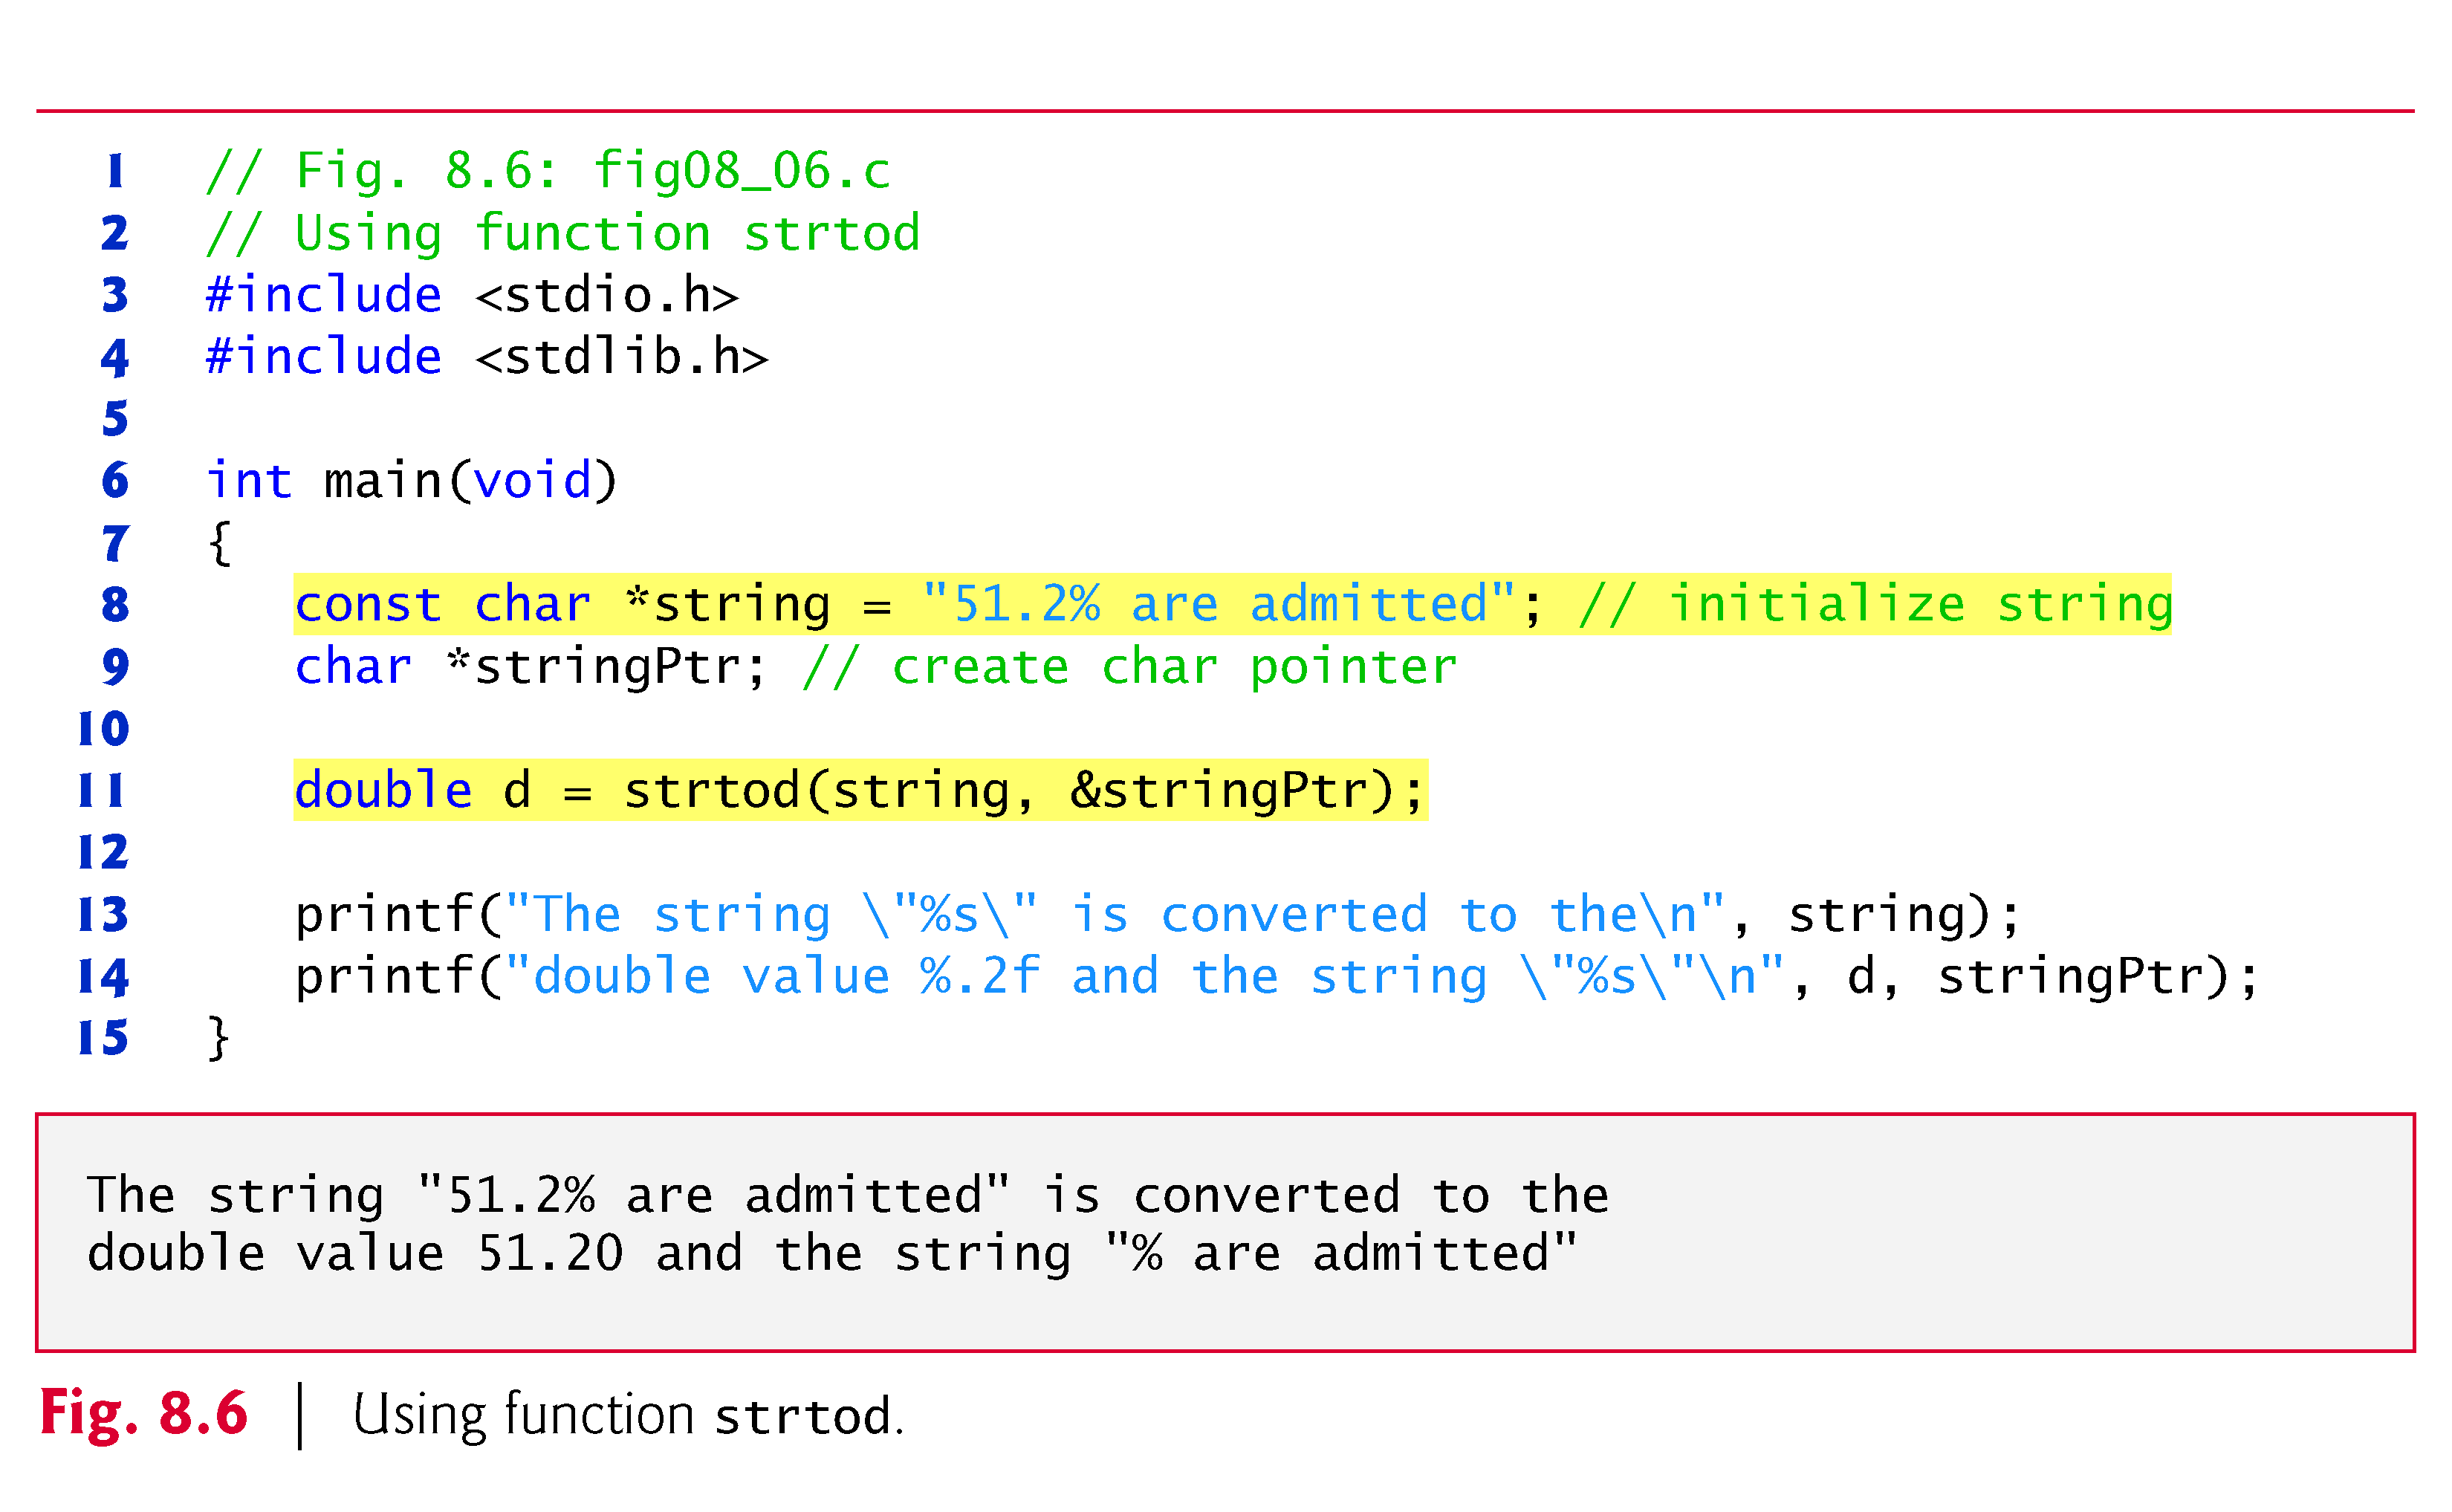
\includegraphics[scale=0.12]{strtod.png}
If \texttt{strtod()} fails to convert a string, it will return \texttt{0}.
\end{frame}

\begin{frame}[fragile=singleslide]{Converting String to \texttt{int}}
Similarly to \texttt{strtod()}, \texttt{stdlib.h} provides a function for converting strings to integers: \texttt{strtol()}
\begin{lstlisting}[style=C]
long int strtol(const char *str, char **endptr, int base);
\end{lstlisting}
\begin{itemize}
\item Key Differences:
\begin{itemize}
\item the return type is an 8-byte \texttt{long int}.
\item \texttt{strtol()} accepts a third argument, the base of the number we are interpretting.
\begin{itemize}
\item 0 $\leftarrow$ Octal, Decimal or Hexadecimal
\item 2-32 $\leftarrow$ The base indicated.
\item Bases higher than 10 use alphabetic characters in the same manner as Hexadecimal.  
\end{itemize}
\end{itemize}
\end{itemize}
\end{frame}

\begin{frame}{Variations on a Theme in D Minor}
There are a number of conversion functions that work in a similar manner. \\ 
\begin{center}
\begin{tabular}{| l | c |}
\hline
Function & Converts String To... \\ \hline
\texttt{strtod()} & \texttt{double} \\ \hline
\texttt{strtof()} & \texttt{float} \\ \hline
\texttt{strtol()} & \texttt{long int} \\ \hline
\texttt{strtoul()} & \texttt{unsigned long int} \\ \hline
\texttt{strtoll()} & \texttt{long long int} \\ \hline
\texttt{strtoull()} & \texttt{unsigned long long int} \\ \hline
\end{tabular}
\end{center}
\begin{itemize}
\item Note the absence of functions to convert to \texttt{int} and \texttt{short}
\item This is possible directly using the unsafe \texttt{atoi()} function.
\item \texttt{atoi()} is unnecessary, as \texttt{strtol()} can be easily type-cast to either \texttt{int} or \texttt{short}.
\end{itemize}
\end{frame}

\begin{frame}[fragile=singleslide]{Converting Things to Strings}
Now that we know how to read numeric values from strings, the question remains, how do we write numeric values into strings?
\begin{itemize}
\item Trick Question! We've been doing this all along!
\item \texttt{printf()} writes to \texttt{stdout}, but \texttt{snprintf()} writes to a specified memory address.
\end{itemize}
\begin{lstlisting}[style = C]
int snprintf(char *str, size_t size, const char *format, ...);
\end{lstlisting}
\begin{itemize}
\item \texttt{str} is a pointer to the memory address the characters will be written to
\item \texttt{size} sets a maximum number of characters to write.
\begin{itemize}
\item Remember to leave enough space in both of the above for null termination! 
\end{itemize}
\item Every argument past the second is used precisely the same as \texttt{printf()}.
\end{itemize}
\end{frame}


\begin{frame}[fragile=singleslide]{Converting Things to Strings (cont.)}
\begin{itemize}
\item The return value of \texttt{snprintf()} is the size of the format string after substitution.  
\begin{itemize}
\item Note, that this may be distinct from the size of the string written into memory.
\item This means that we can check to see if the string had to be truncated by comparing the input size to the output size. 
\end{itemize}
\end{itemize}
\begin{lstlisting}[style = C]
int i = 1337;
int size = (int)((ceil(log10(i))+1);
char *buffer = (char*) malloc(size*sizeof(char)); 
int j = snprintf(buffer, size, "%d", i); 
if (j > size) {
	printf("Write operation was truncated!");
}
\end{lstlisting}
\end{frame}

\section[string.h]{String Manipulations}
\begin{frame}{String.h: Manipulation Tactics}
\center
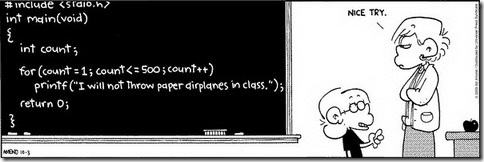
\includegraphics[scale=0.8]{foxtrot.jpg}
\end{frame}

\begin{frame}[fragile=singleslide]{Data Duplication with \texttt{strcpy()}}
Have you ever wanted to copy a string?  Well \texttt{strcpy()} and \texttt{strncpy()} are the functions for you! 
\begin{lstlisting}[style = C]
char *strcpy(char *s1, const char *s2);
char *strncpy(char *s1, const char *s2, size_t n);
\end{lstlisting}
\begin{itemize}
\item Both take the string stored at \texttt{s2} and copy it to \texttt{s1}.
\item The extra argument in \texttt{strncpy()} is similar to \texttt{size} in \texttt{snprintf()}.  
\begin{itemize}
\item \texttt{strncpy()} will copy \emph{at most} \texttt{n} characters.
\item This guards against buffer overflow, making \texttt{strncpy()} the ``safe version'' of \texttt{strcpy()}.
\end{itemize}
\item Once again, \emph{you} must make sure:
\begin{itemize}
\item \texttt{s1} is large enough to contain \texttt{s2}
\item \texttt{n} takes null termination into account.  
\end{itemize}
\end{itemize}
\end{frame}

\begin{frame}[fragile=singleslide]{Yet More Functions!}
\begin{lstlisting}[style = C]
char *strcat(char *s1, const char *s2);
char *strncat(char *s1, const char *s2, size_t n);
size_t strlen(const char *s);
\end{lstlisting}
\begin{itemize}
\item \texttt{strcat()} usage is similar to \texttt{strcpy()}
\begin{itemize}
\item The null character terminating \texttt{s1} is overwritten with the first character of \texttt{s2}.  
\end{itemize}
\item \texttt{strlen()} accepts a string and produces the number of characters in it, null character excluded.  
\end{itemize}
\end{frame}

\begin{frame}[fragile=singleslide]{My String's Better Than Your String... \texttt{strcmp}}
Ever needed to tell if two strings are the same string? Try \texttt{strcmp()} on for size! 
\begin{lstlisting}[style = C]
int strcmp(const char *s1, const char *s2);
int strncmp(const char *s1, const char *s2, size_t n);
\end{lstlisting}
\begin{itemize}
\item Inputs are the same as previously
\item Compares the characters in each string sequentially and returns:
\begin{itemize}
\item \texttt{0} if the strings are the same.
\item A value less than 0 if s1 is ``less than'' s2
\item A value greater than 0 if s1 is ``greater than'' s2.
\end{itemize}
\item In this context, strings are ordered by the ASCII values of their characters, using alphabetization rules.
\item This is known as \textbf{Lexographical Ordering.}
\end{itemize}
\end{frame}

\begin{frame}{A Table with Equivalent Python Operations}
\center
\begin{tabular}{| l | c |}
\hline 
C function & Rough Python Equivalent \\ \hline
\texttt{strtol()} & \texttt{int(myString)} \\ \hline
\texttt{snprintf()} & \texttt{str(myInt)} \\ \hline
\texttt{strcpy()} & \texttt{copy.deepcopy(foo)} \\ \hline
\texttt{strcat()} & \texttt{foo + bar} \\ \hline
\texttt{strlen()} & \texttt{len(foo)} \\ \hline
\texttt{strcmp()} & [\texttt{==}, \texttt{\textless}, \texttt{\textgreater}, etc.] \\ \hline
\texttt{strchr()} & \texttt{foo.index(bar)} \\ \hline
\texttt{strtok()} & \texttt{foo.split(bar)} \\ \hline
\end{tabular}
\end{frame}

% \begin{frame}{Surely This is Generalizable.}
% Given that in C, data types as a concept are somewhat ephemeral, it should be the case that the above operations on \texttt{char*}s should be reasonably generalizable.
% \begin{itemize}
% \item \texttt{string.h} contains a set of memory operations which are highly similar to the operations on strings previously discussed. 
% \item Rather than accepting and returning \texttt{char*} pointers, these functions use \texttt{void*} pointers.  
% \end{itemize}
% \begin{tabular}{| l | c | c |}
% \hline 
% C function & C String Equivalent & Rough Python Equivalent \\ \hline
% \texttt{memcpy()} & \texttt{strcpy()} & \texttt{copy.deepcopy(foo)} \\ \hline
% \texttt{memcmp()} & \texttt{strcmp()} & [\texttt{==}, \texttt{\textless}, \texttt{\textgreater}, etc.] \\ \hline
% \texttt{memchr()} & \texttt{strchr()} & \texttt{foo.index(bar)} \\ \hline
% \end{tabular}
% \end{frame}

\section[Formatting]{Advanced Formatting}
\begin{frame}{Formatting: What can't it do?}
Up to this point, we have only briefly touched on the advanced features of the string formatting tag \texttt{\%}.  We will discuss the following features:
\begin{itemize}
\item Rounding of floating point numbers, and displaying a specified number of decimal places.
\item Aligning columns of numbers
\item Right and Left Justification of outputs
\item Exponential formats for floating point numbers
\item Fixed field widths for various data types
\end{itemize}
All of the format specifiers we are about to discuss are used in \texttt{printf()}, \texttt{scanf()} and their cousins.
\end{frame}

\begin{frame}{Format Specifiers for Integer Formats}
\center
\includegraphics[scale=0.12]{integers.png}
\end{frame}

\begin{frame}{Printing Integers in Various Ways}
\center
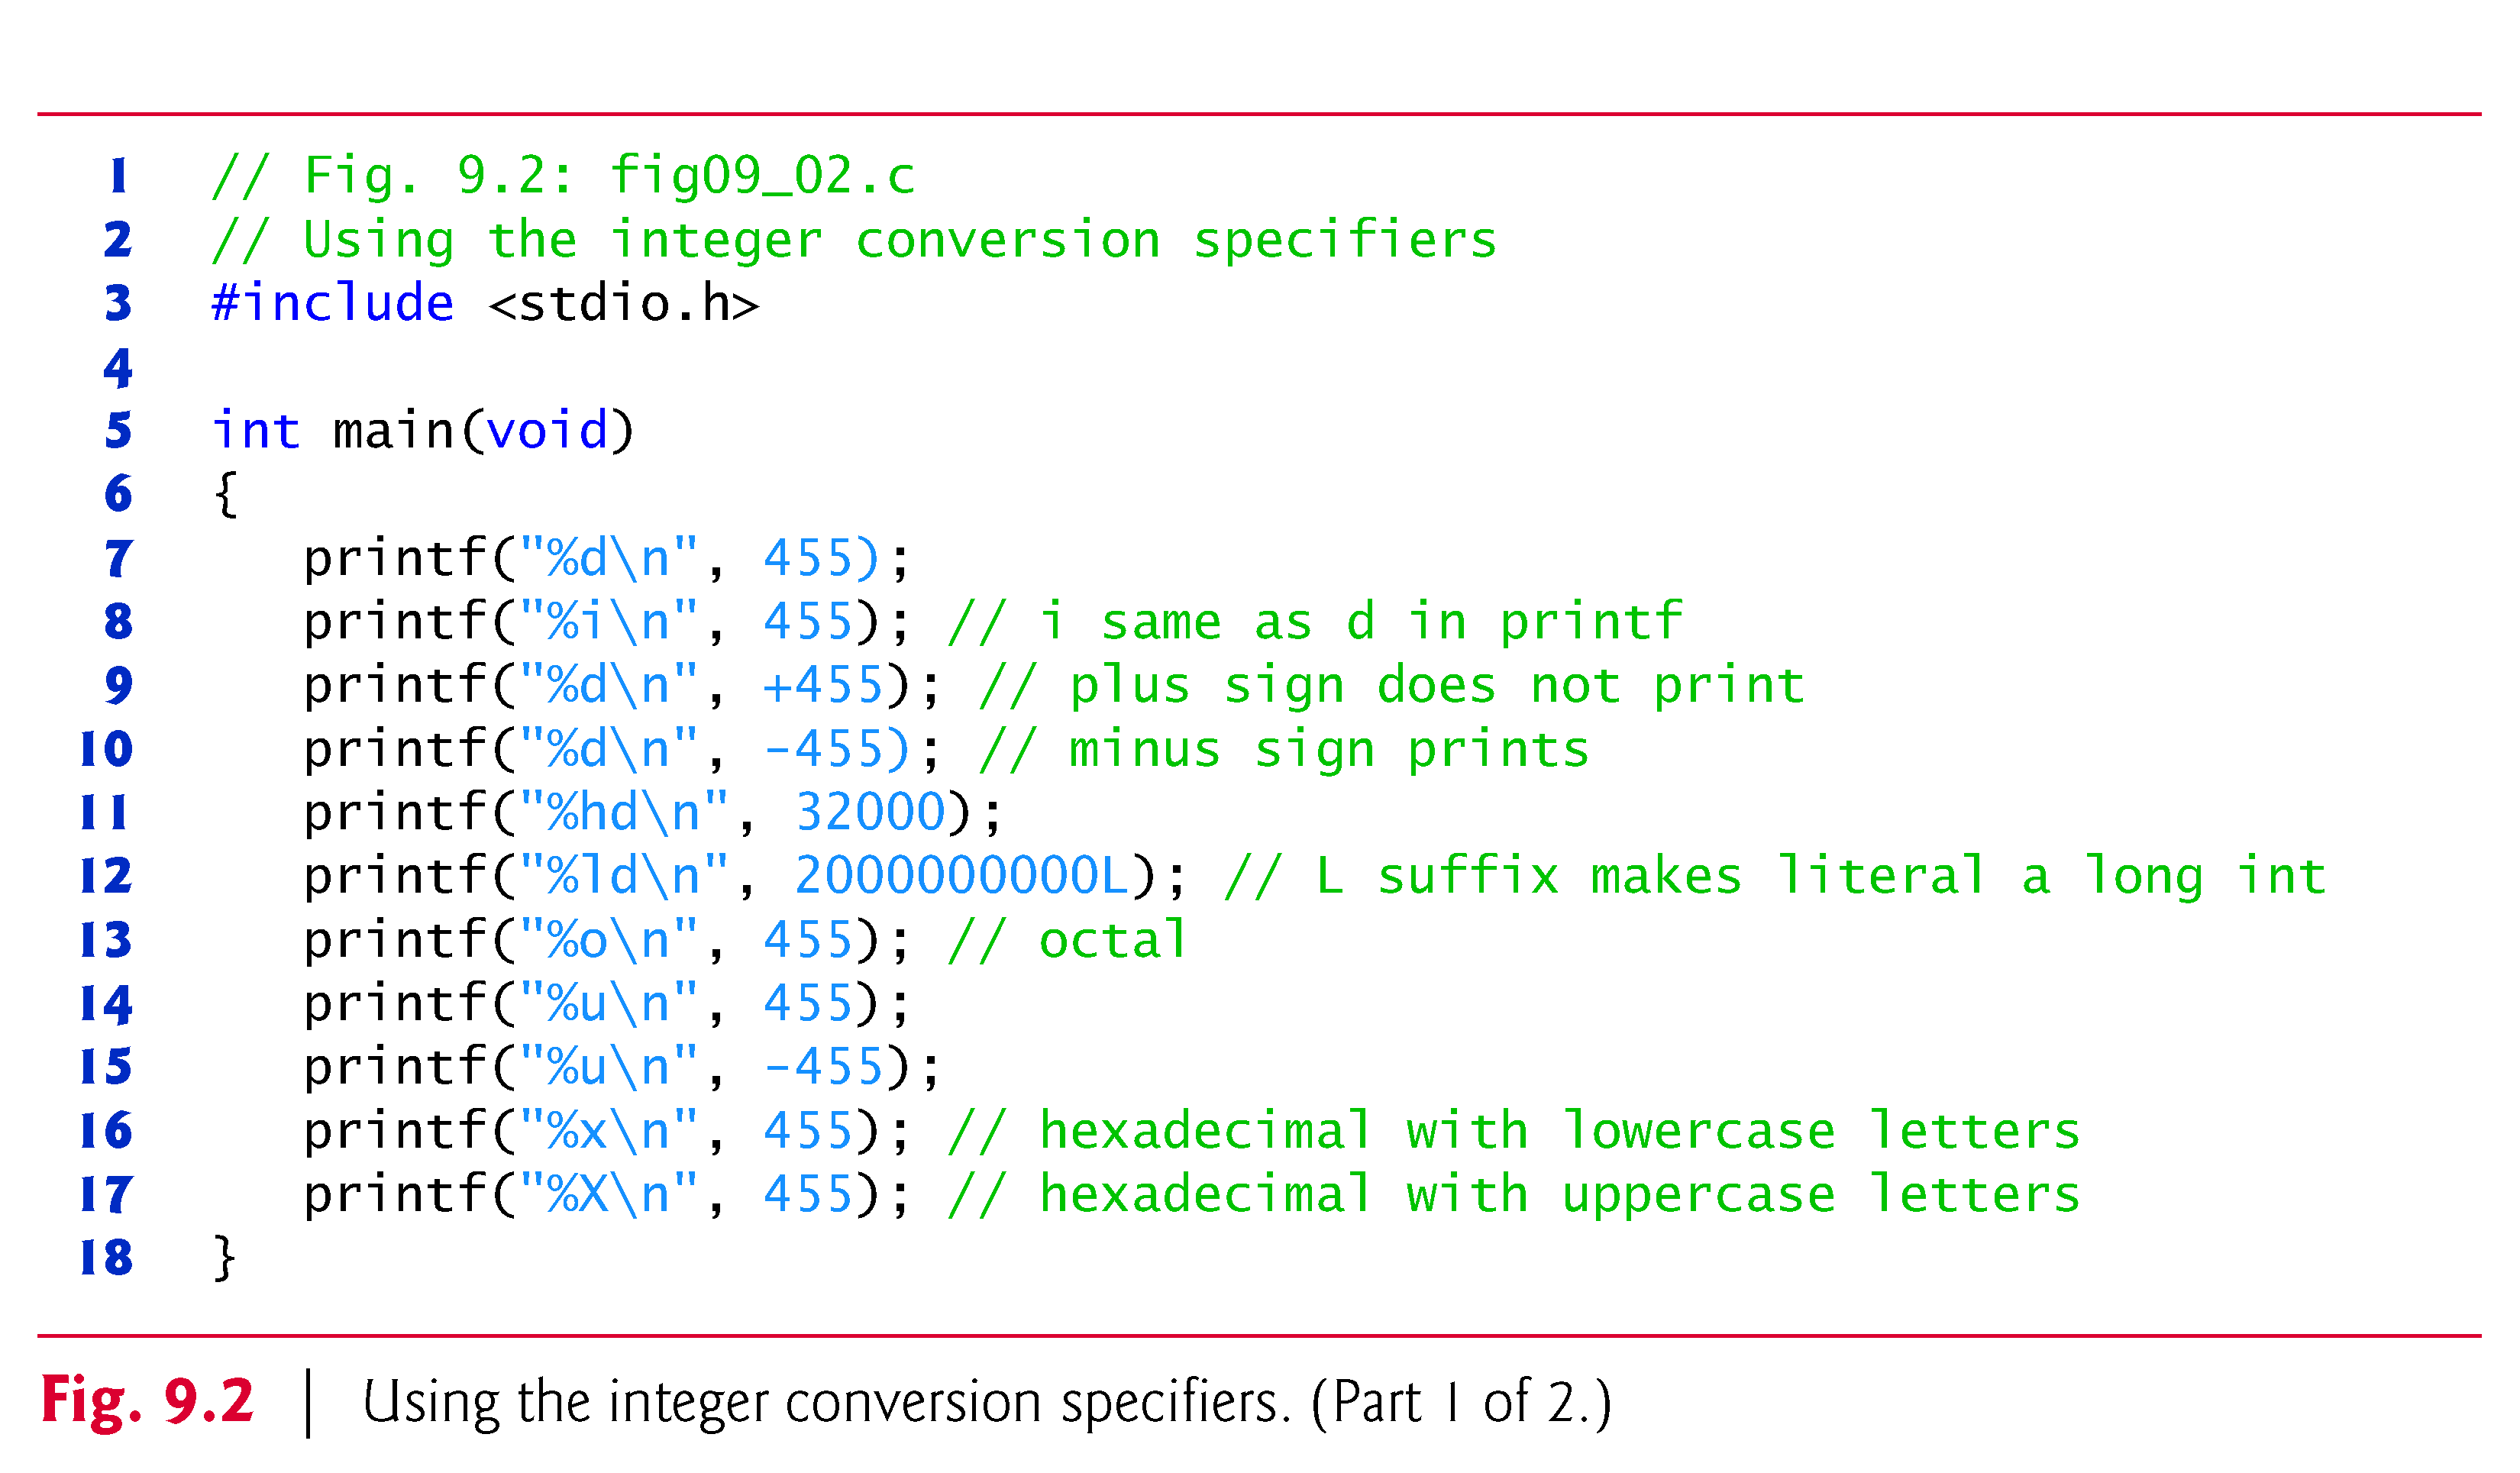
\includegraphics[scale=0.12]{intExample1.png}
\end{frame}

\begin{frame}{Printing Integers in Various Ways (cont.)}
\center
\includegraphics[scale=0.35]{intExample2.png}
\flushleft
Things of note:
\begin{itemize}
\item The literal \texttt{2000000000L} is cast as a \texttt{long int} with the suffix \texttt{L}.
\item A negative number, interpreted as an unsigned integer, is very large! 
\begin{itemize}
\item This is because negative numbers are stored using \textbf{Two's Complement}, which we'll be discussing soon.
\end{itemize}
\end{itemize}
\end{frame}

\begin{frame}{Printing Floating Point Numbers}
\center
\includegraphics[scale=0.12]{floats.png}
\end{frame}

\begin{frame}{Example Floats}
\center
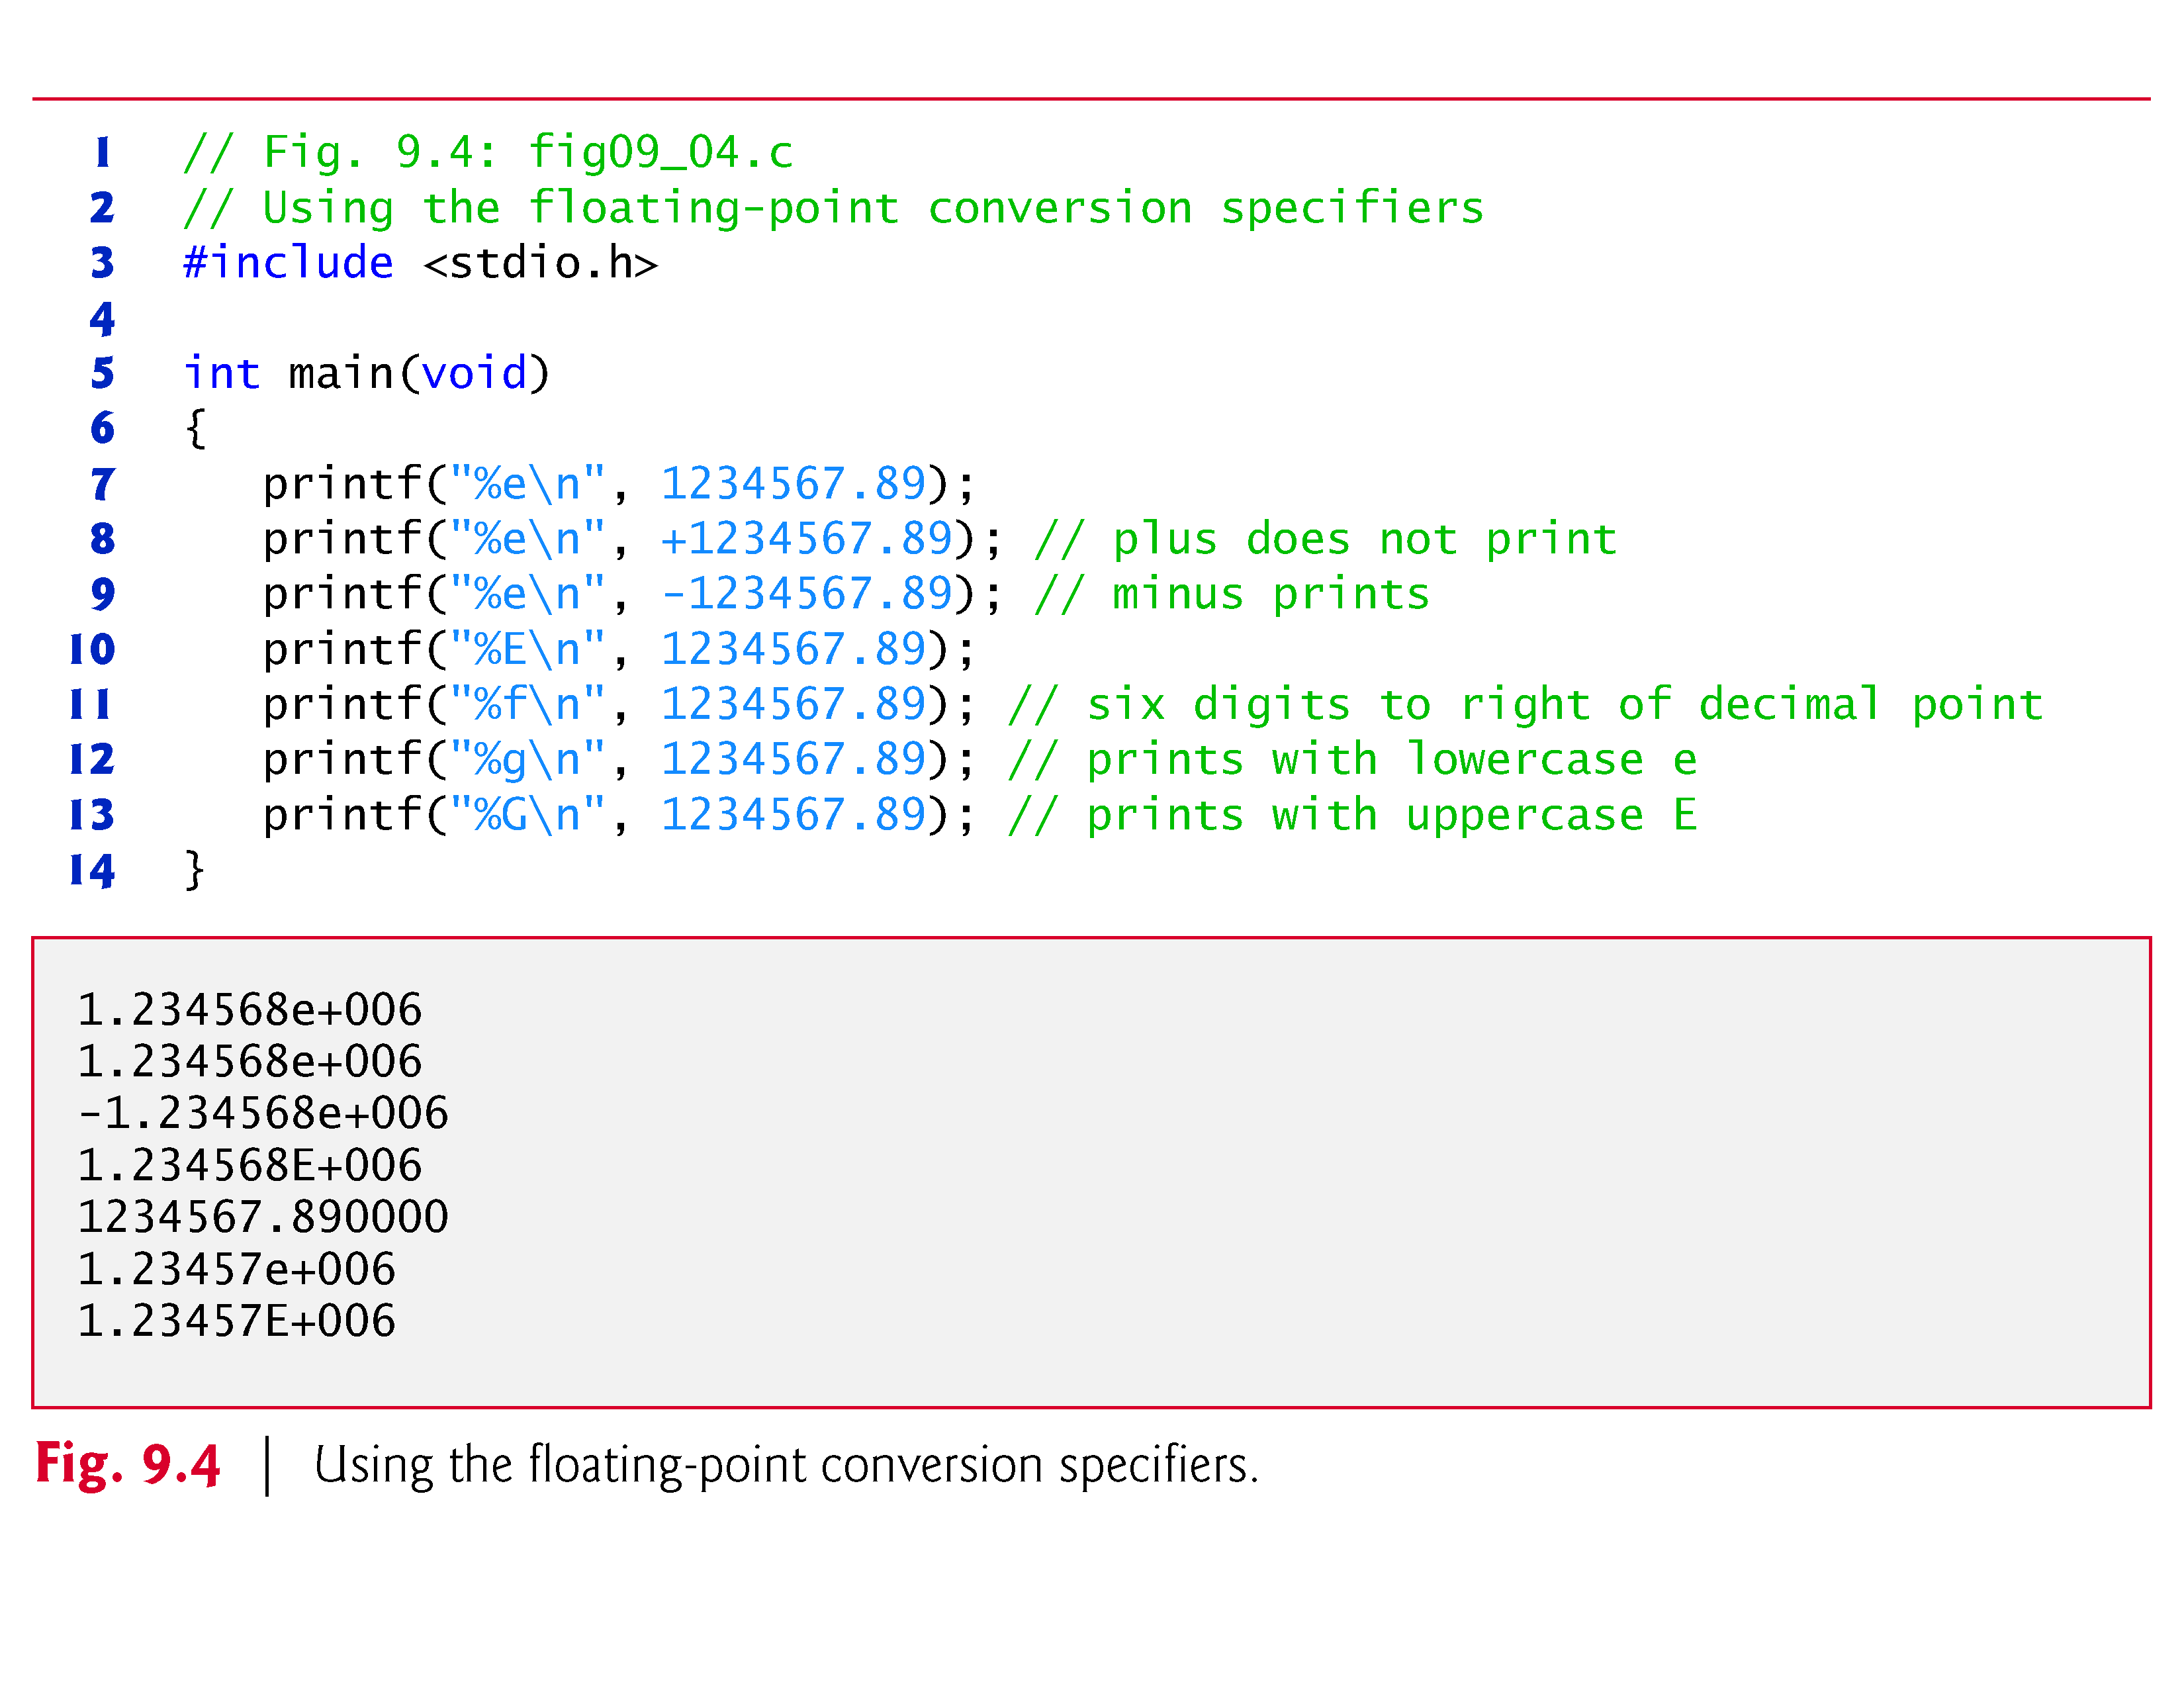
\includegraphics[scale=0.34]{floatsExample.png}
\end{frame}

\begin{frame}{Floating Some Ideas...}
\begin{itemize}
\item \texttt{e} and \texttt{f} show six digits of precision by default.
\item \texttt{f} will always print at least one digit to the left of the decimal point.  
\item \texttt{g} will select \texttt{e} if the exponent would be greater than the specified precision (default 6) or less than -4, and \texttt{f} otherwise. 
\item \texttt{g} does not print trailing zeroes.  
\item \texttt{e} and \texttt{g} display \emph{rounded} values, \texttt{f} displays \emph{truncated} values.  
\end{itemize}
Random Trivia: You can print the \texttt{\%} character with either \texttt{\%\%}.  Note that \texttt{\textbackslash \%} doesn't work.
\end{frame}

\begin{frame}{Working with Field Widths}
Ever been bummed out because getting C to print a table of values with properly aligned numbers is hard?  Fear no more! 
\begin{itemize}
\item Inserting an integer value between the \texttt{\%} character and the format specifier sets the \textbf{field width}. 
\item Data will normally be \emph{right justified} within this field. 
\item Field widths may be used with all format specifiers.  
\item If your field width is too narrow for your data, that data will ``overhang'' the specified width, rather than being truncated.  
\end{itemize}
\end{frame}

\begin{frame}{Field Widths}
\center
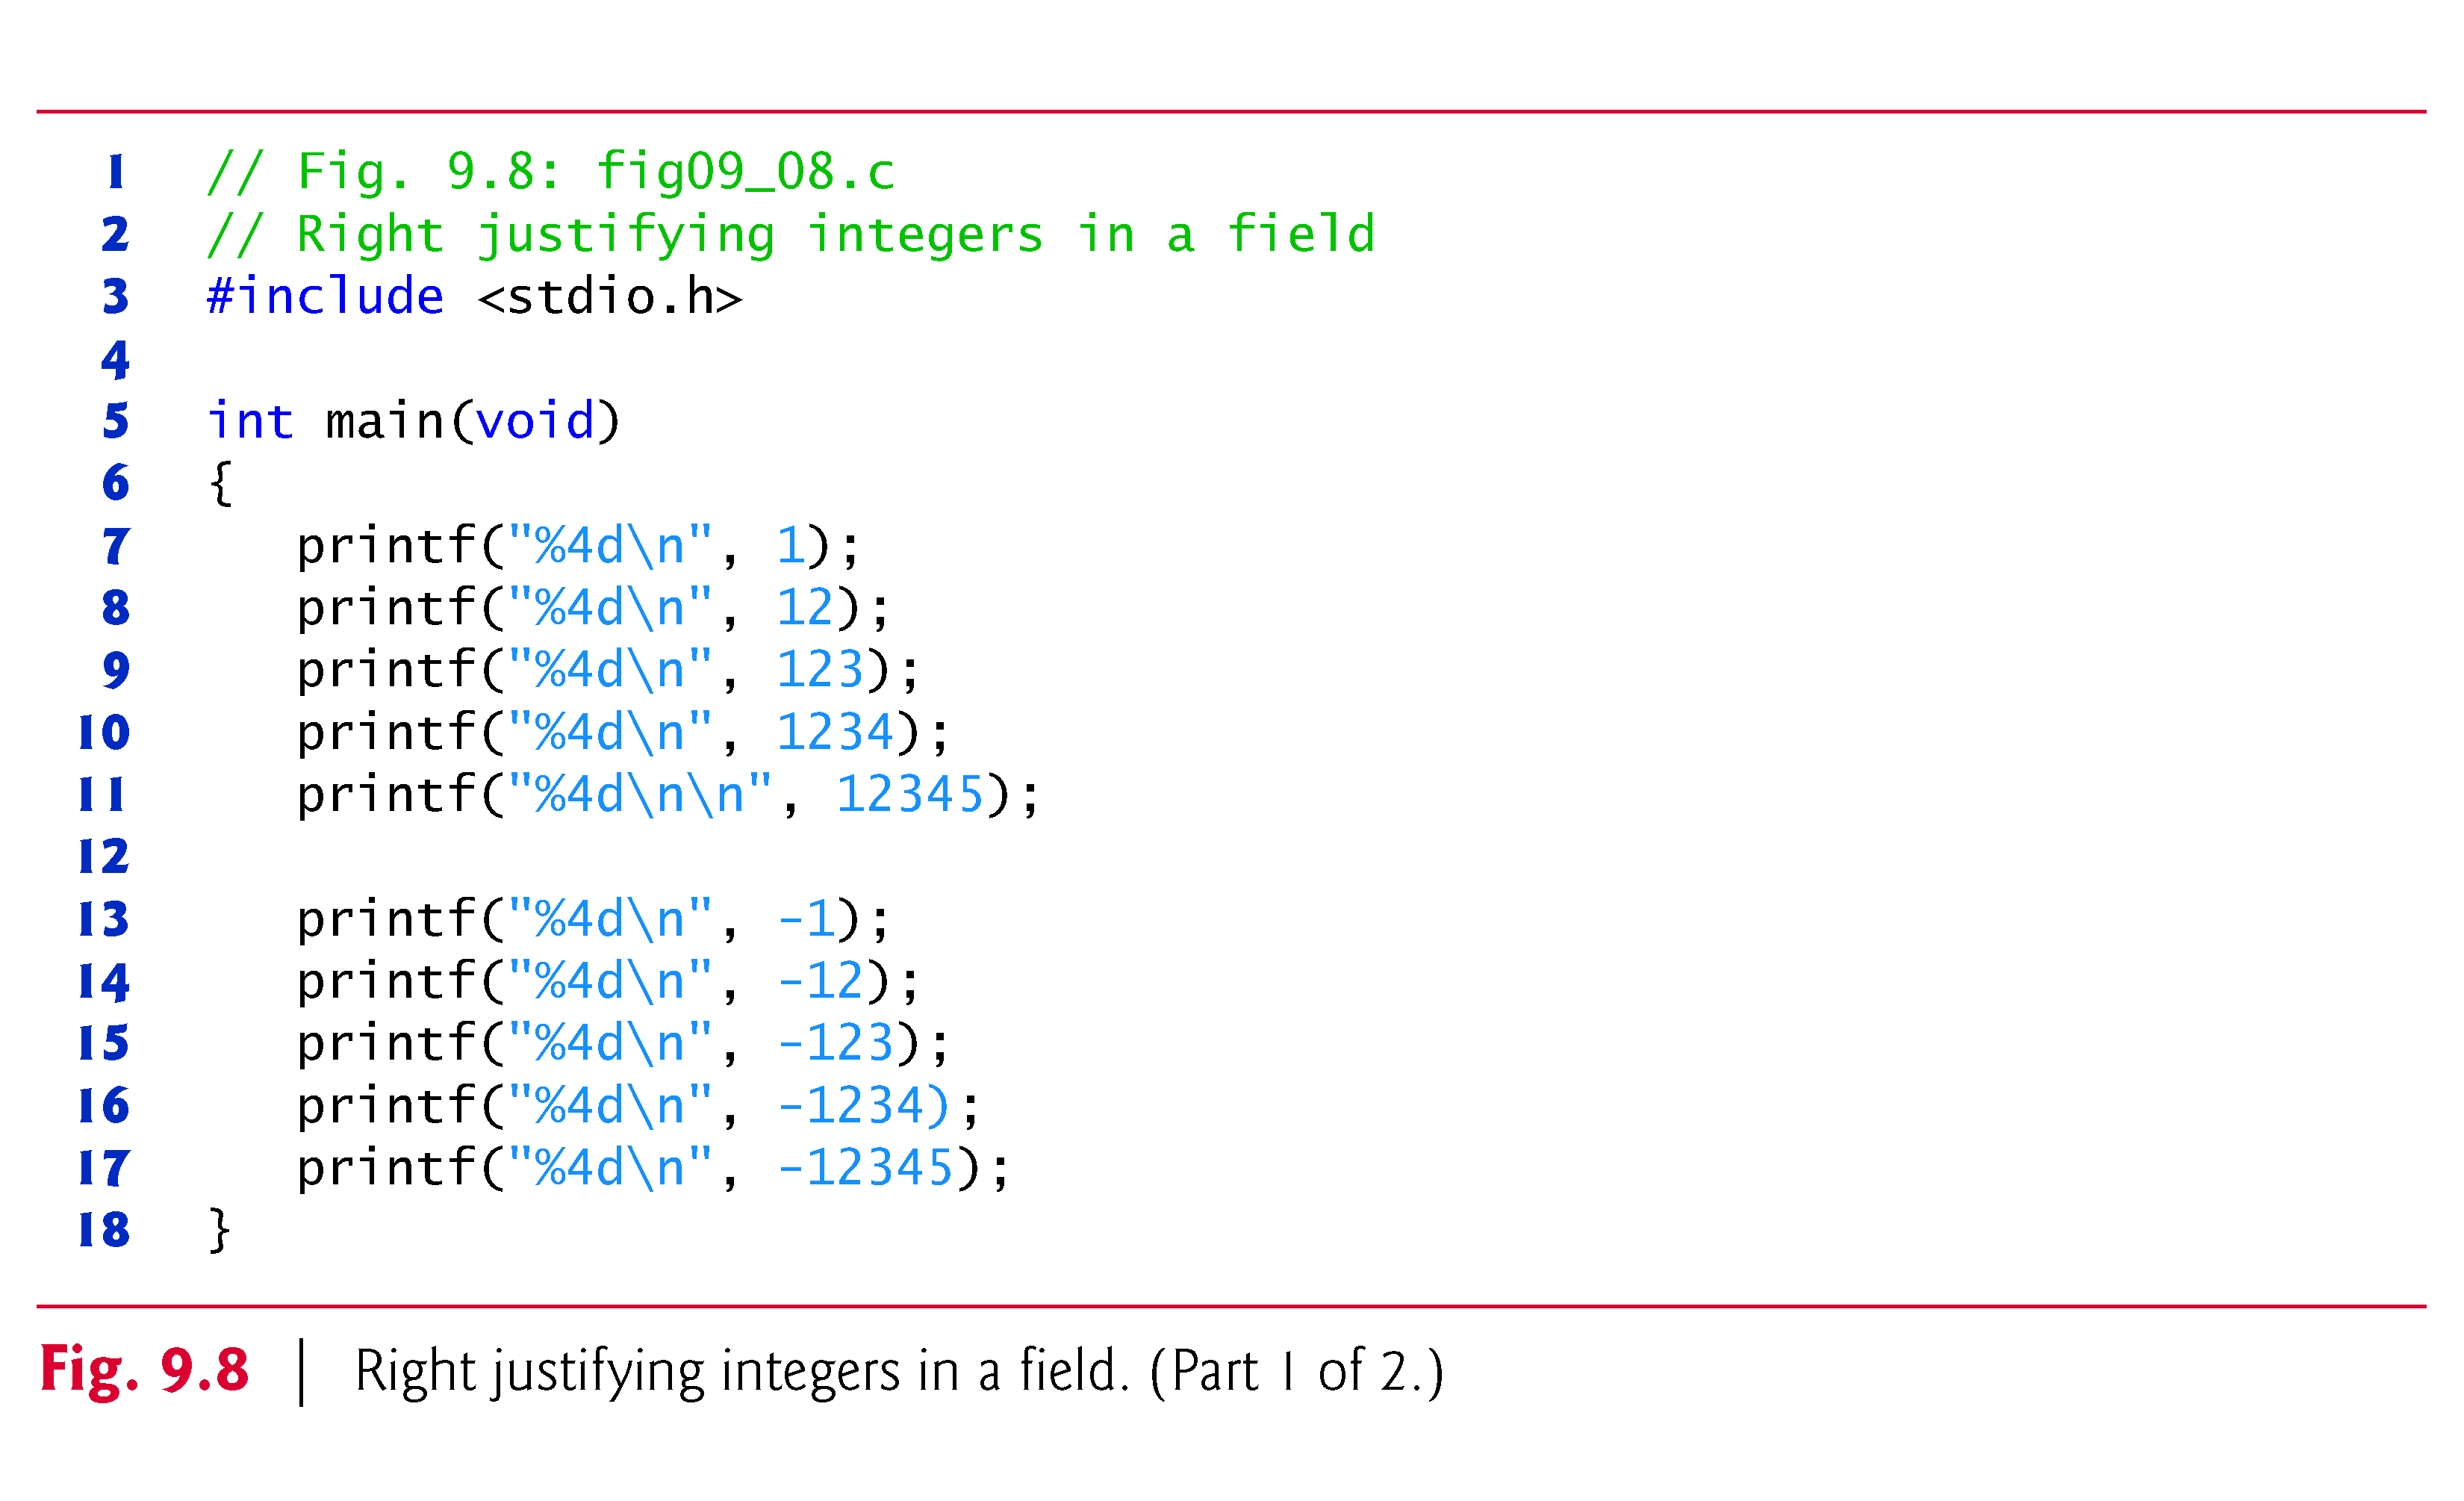
\includegraphics[scale=0.12]{width.png}
\end{frame}

\begin{frame}{Field Widths (cont.)}
\center
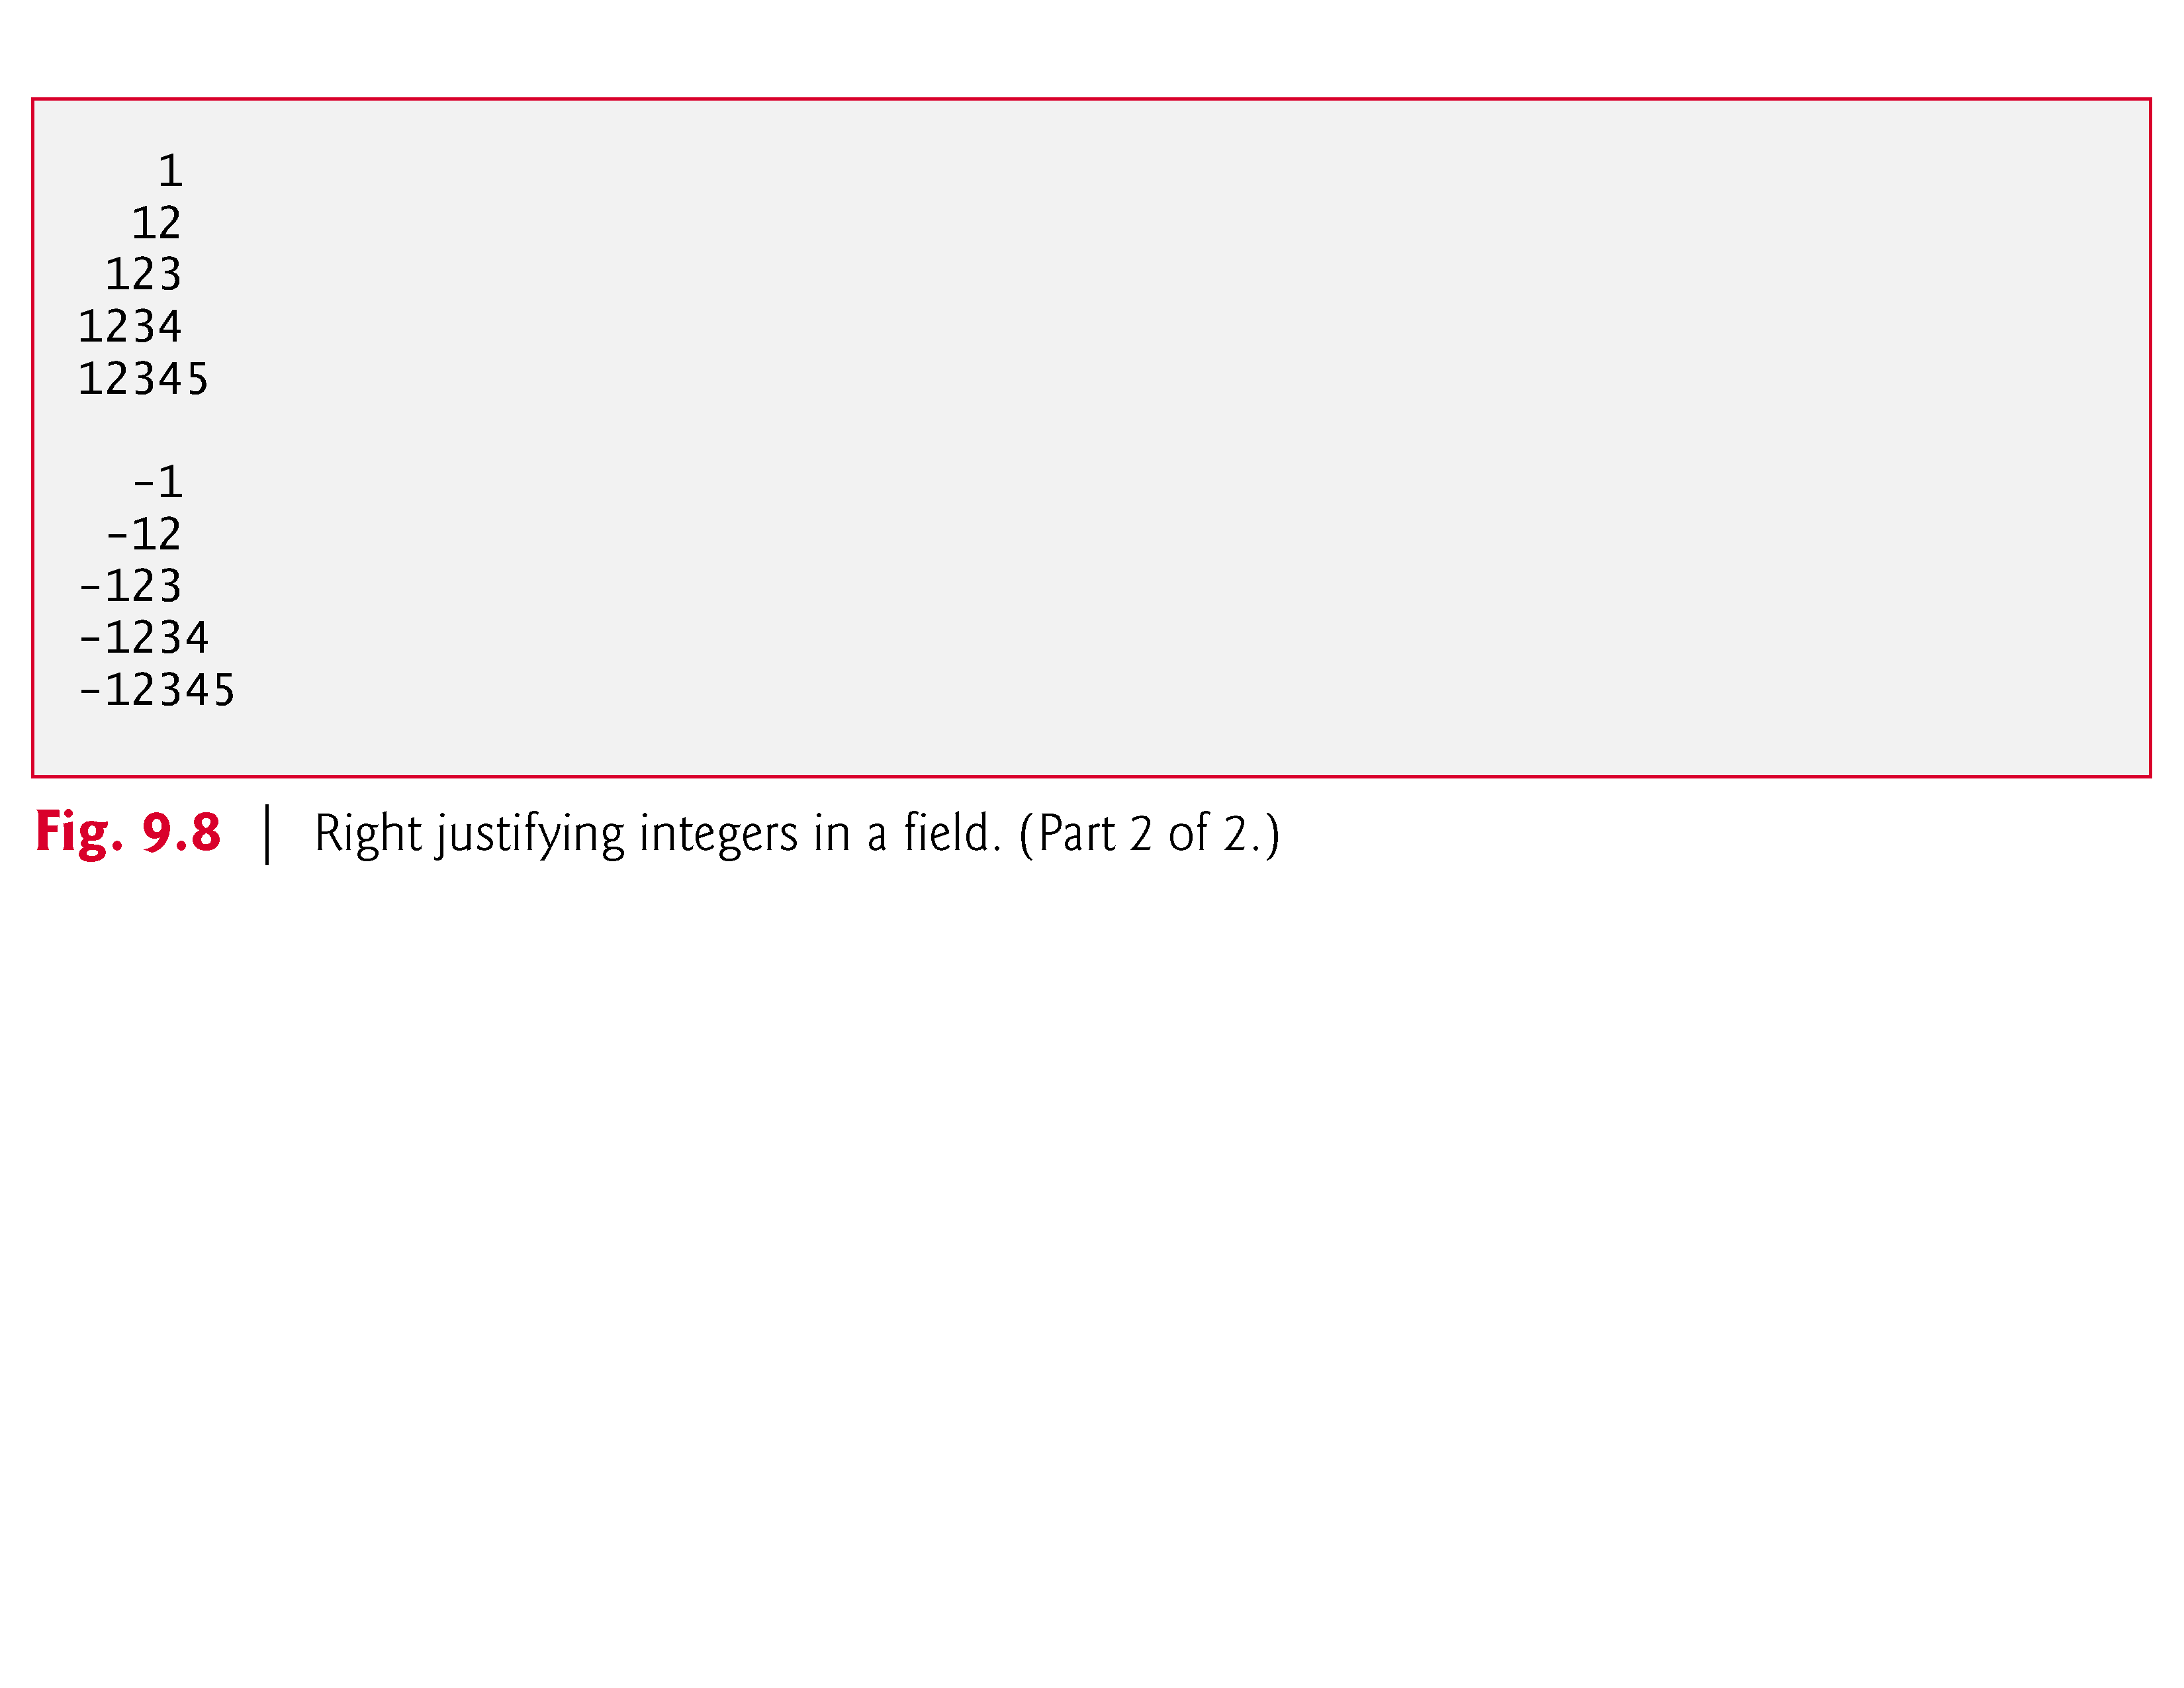
\includegraphics[scale=0.35]{width2.png}
\end{frame}

\begin{frame}{Field Widths with Precision}
We can specify various things for different data types using the \texttt{.X} format tag.
\begin{itemize}
\item When applied to \texttt{int}s, leading zeros are included instead of spaces, to fill the field width.
\item When applied to \texttt{float}s, this controls the number of decimal places that are displayed (i.e., the precision).
\item When applied to strings, this sets the number of characters to display.  The rest of the string will be truncated.
\begin{itemize}
\item The \texttt{\%s} tag looks for a terminating null character.
\item If you aren't careful, \texttt{\% s} can produce a segfault! 
\item Using \texttt{\% s} instead of \texttt{\% c} by mistake can also cause this.
\item Specifying a field width is an effective countermeasure against a non-null-terminated string.  
\end{itemize}
\end{itemize}
\end{frame}

\begin{frame}{Let's be Precise About This!}
\center
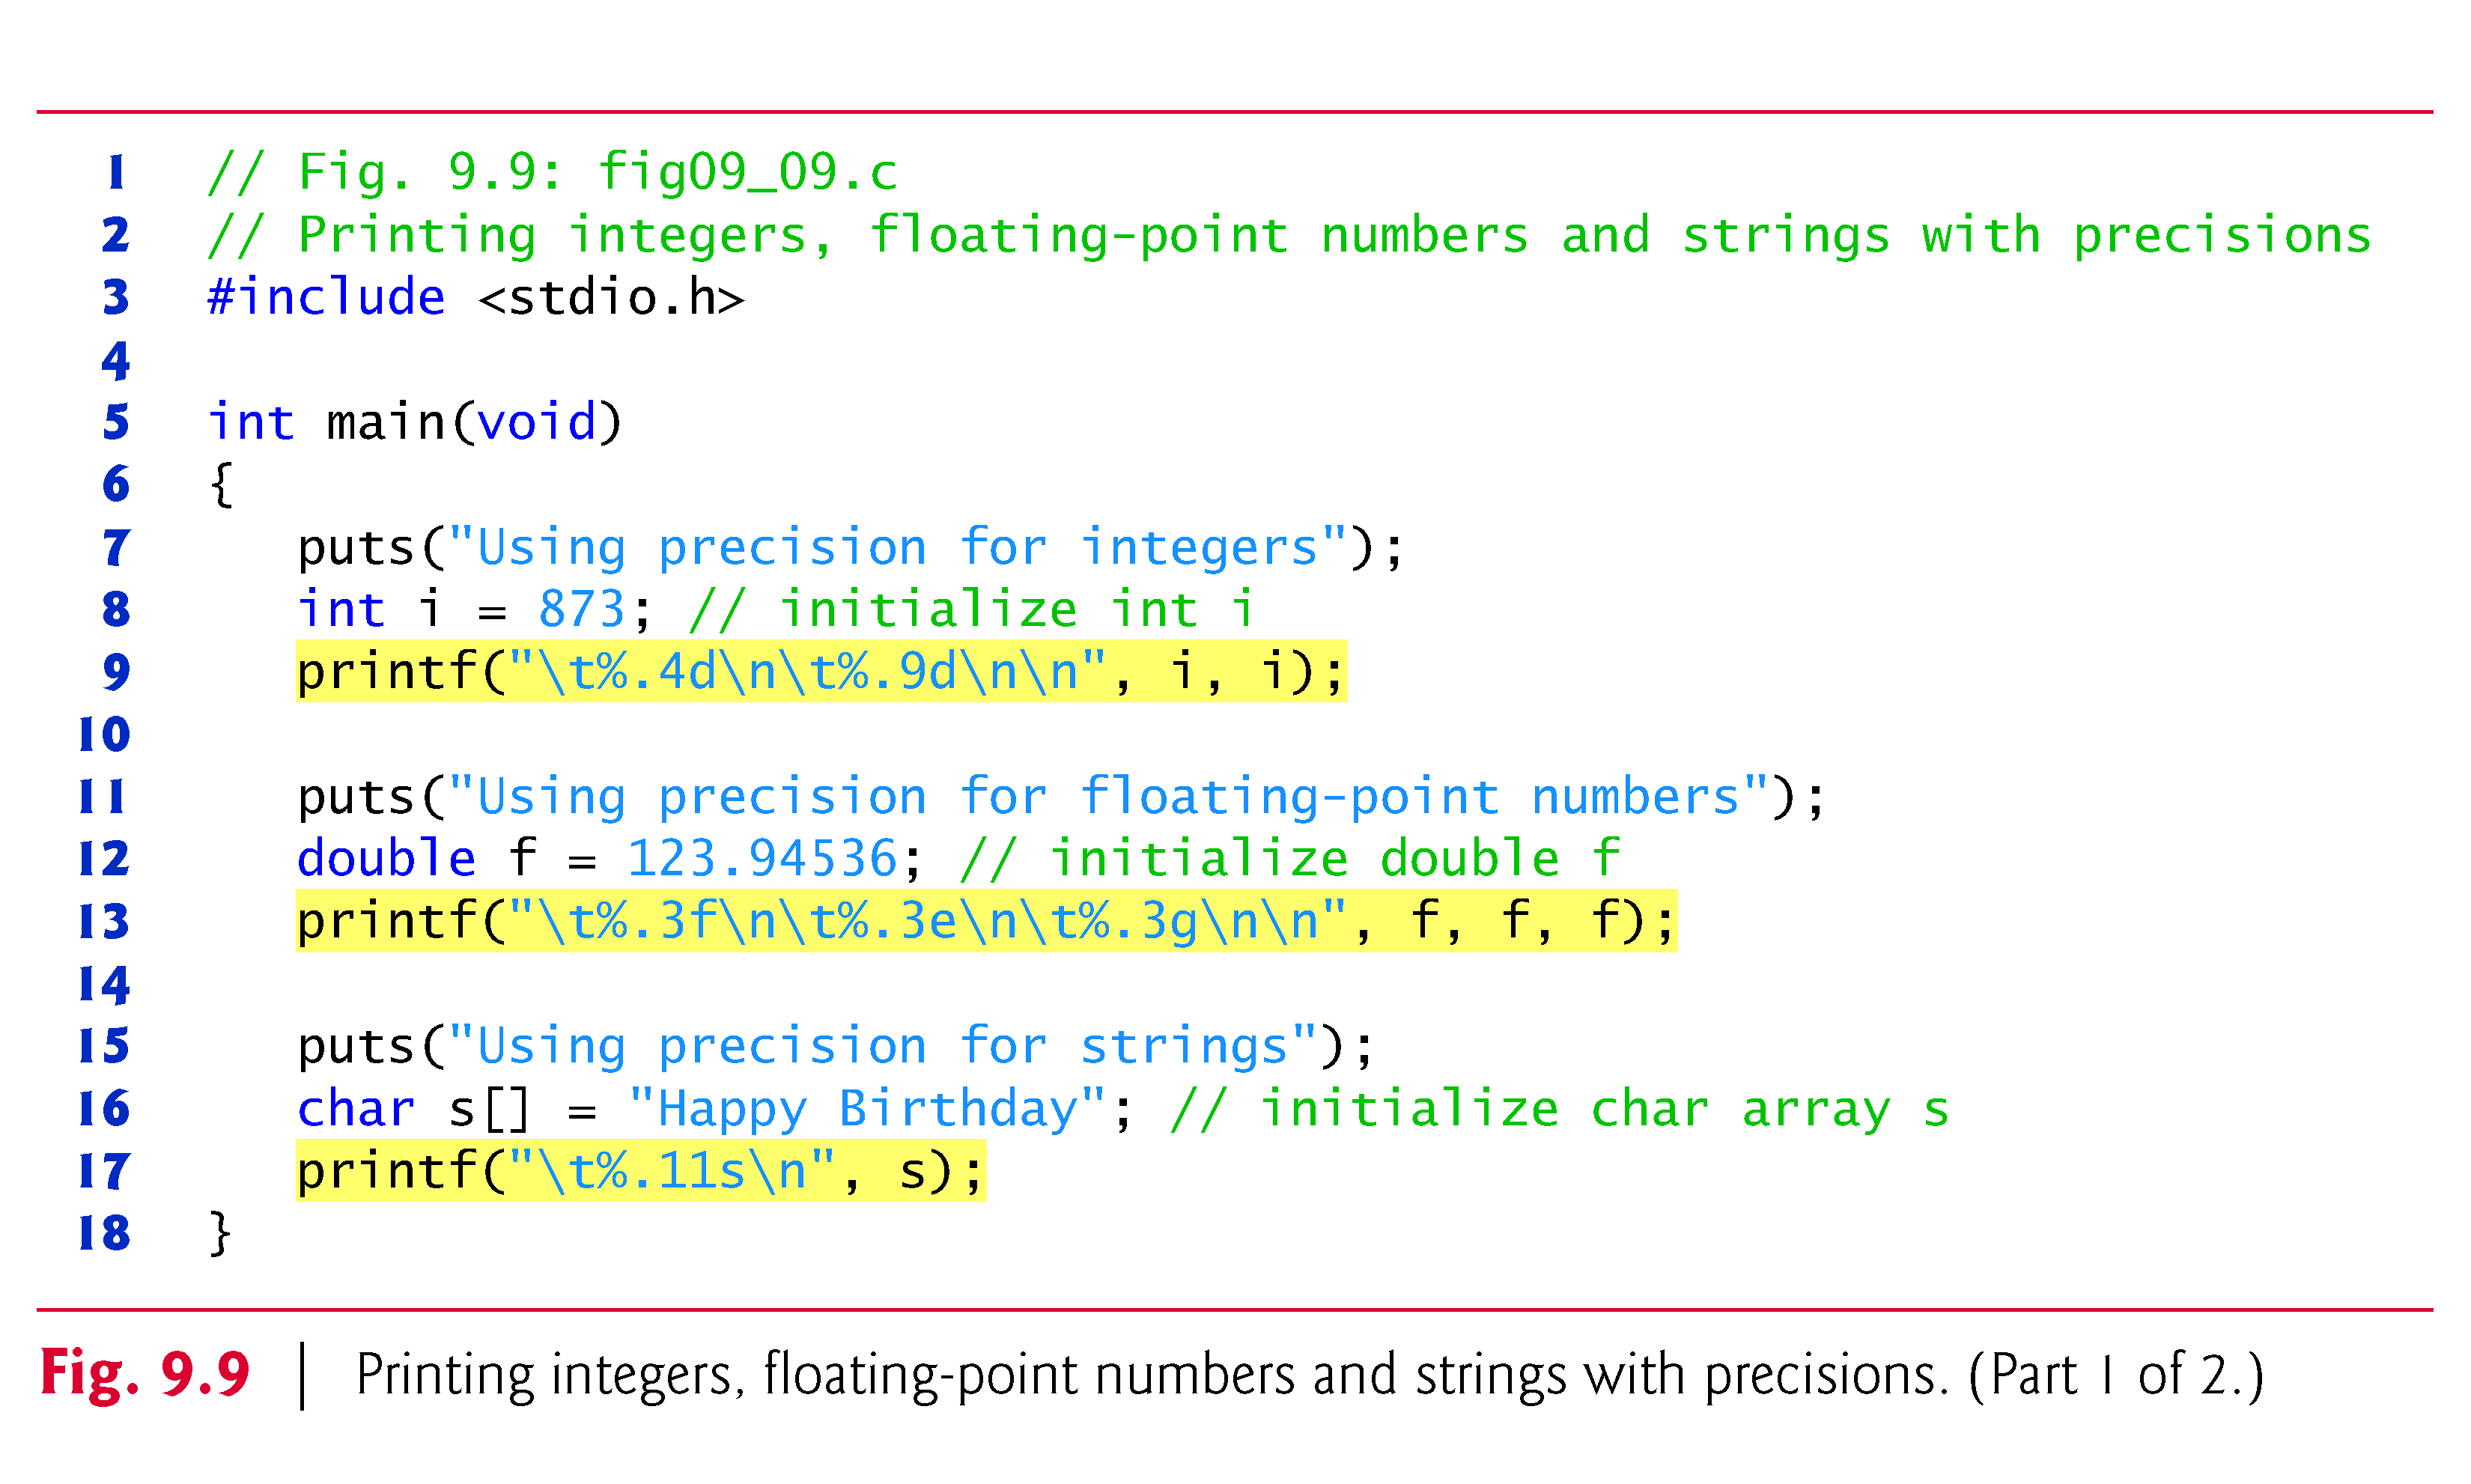
\includegraphics[scale=0.12]{prec.png}
\end{frame}



\begin{frame}[fragile=singleslide]{Let's be Precise About This! (cont.)}
\center
\includegraphics[scale=0.12]{prec2.png}
\flushleft
Field widths and precisions may be used together! 
\begin{lstlisting}[style = C]
printf("%9.6f", 123.456789);
\end{lstlisting}
\hrule
\begin{lstlisting}[style=terminal]
__123.456
\end{lstlisting}
(The underscores above were added to visualize the spaces)
\end{frame}


\begin{frame}{Various Options}
In addition, there are a number of flags that may be included to modify print format.
\center
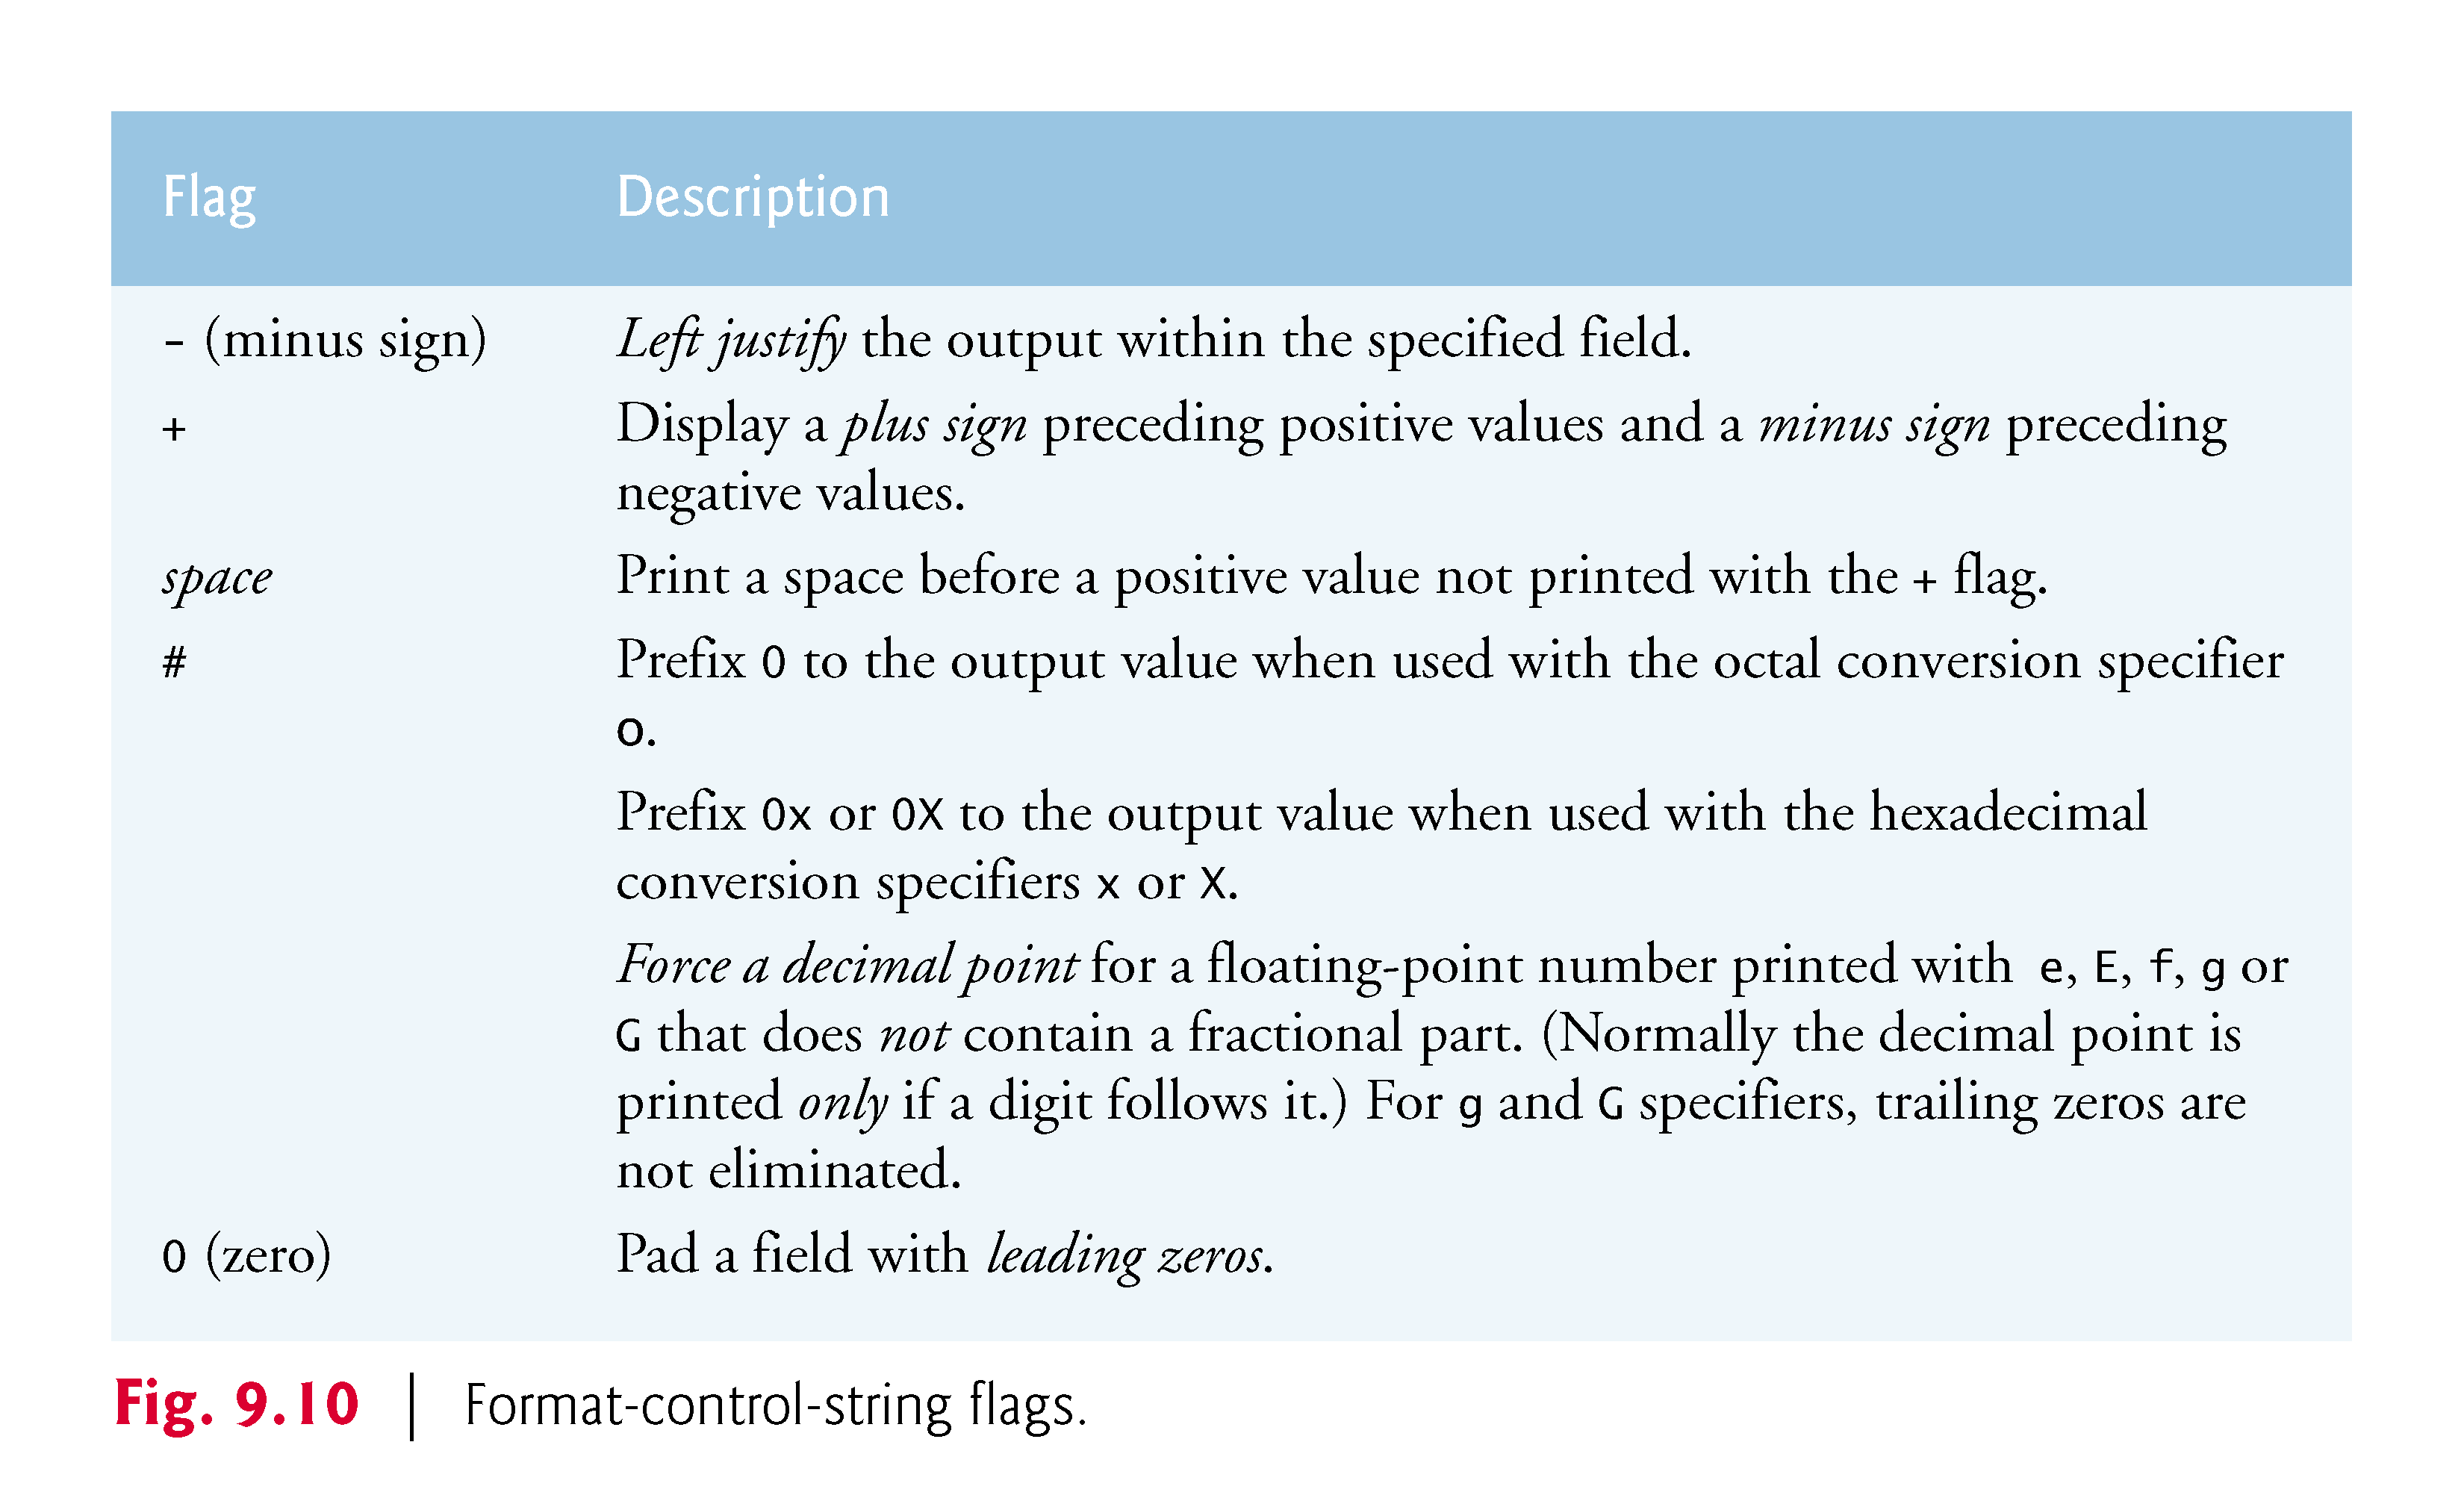
\includegraphics[scale=0.10]{flags.png}
\end{frame}

\section[File I/O]{Permanent Memory Interaction}
% \begin{frame}{Remember Kids, Don't Drink and Code!}
% \center
% \includegraphics[scale=0.3]{comments.png}
% \end{frame}

\begin{frame}{File Operations}
The following five functions are the essential operations for reading from and writing to files.  
\begin{itemize}
\item \texttt{fopen()}, \texttt{fclose()}, \texttt{fscanf()}, \texttt{fread()}, \texttt{fwrite()}, \texttt{fprintf}, \texttt{feof()}
\end{itemize}
Using these files requires knowledge of the \texttt{FILE} structure, which is defined in \texttt{<stdio.h>}.  Think of it as a structure containing all the inforation relevant to a file that is currently being streamed. 
\begin{itemize}
\item It will probably make more sense when we cover \texttt{struct} next week.
\item This section assumes you at least vaguely remember how to do this in python.  
\end{itemize}
\end{frame}

\begin{frame}[fragile=singleslide]{\texttt{fopen()}}
Opening a file stream requires an invokation of \texttt{fopen()}.
\begin{lstlisting}[style=C]
FILE *fopen(const char *filename, const char *mode);
\end{lstlisting}
\begin{itemize}
\item As you may expect, \texttt{filename} is a string, containing the name of the file to be opened.
\begin{itemize}
\item The file may be specified by either absolute or relative addressing.  
\end{itemize}
\item \texttt{mode} is a string specifying, among other things, whether the file will be opened in read or write mode.  
\item The output of this function is a \texttt{FILE} pointer to the data stream object.  You don't have to worry about direct manipulation of this pointer, it is only interacted with via the file operation functions.  
\end{itemize}
\end{frame}

\begin{frame}{Modus Operandi}
\center
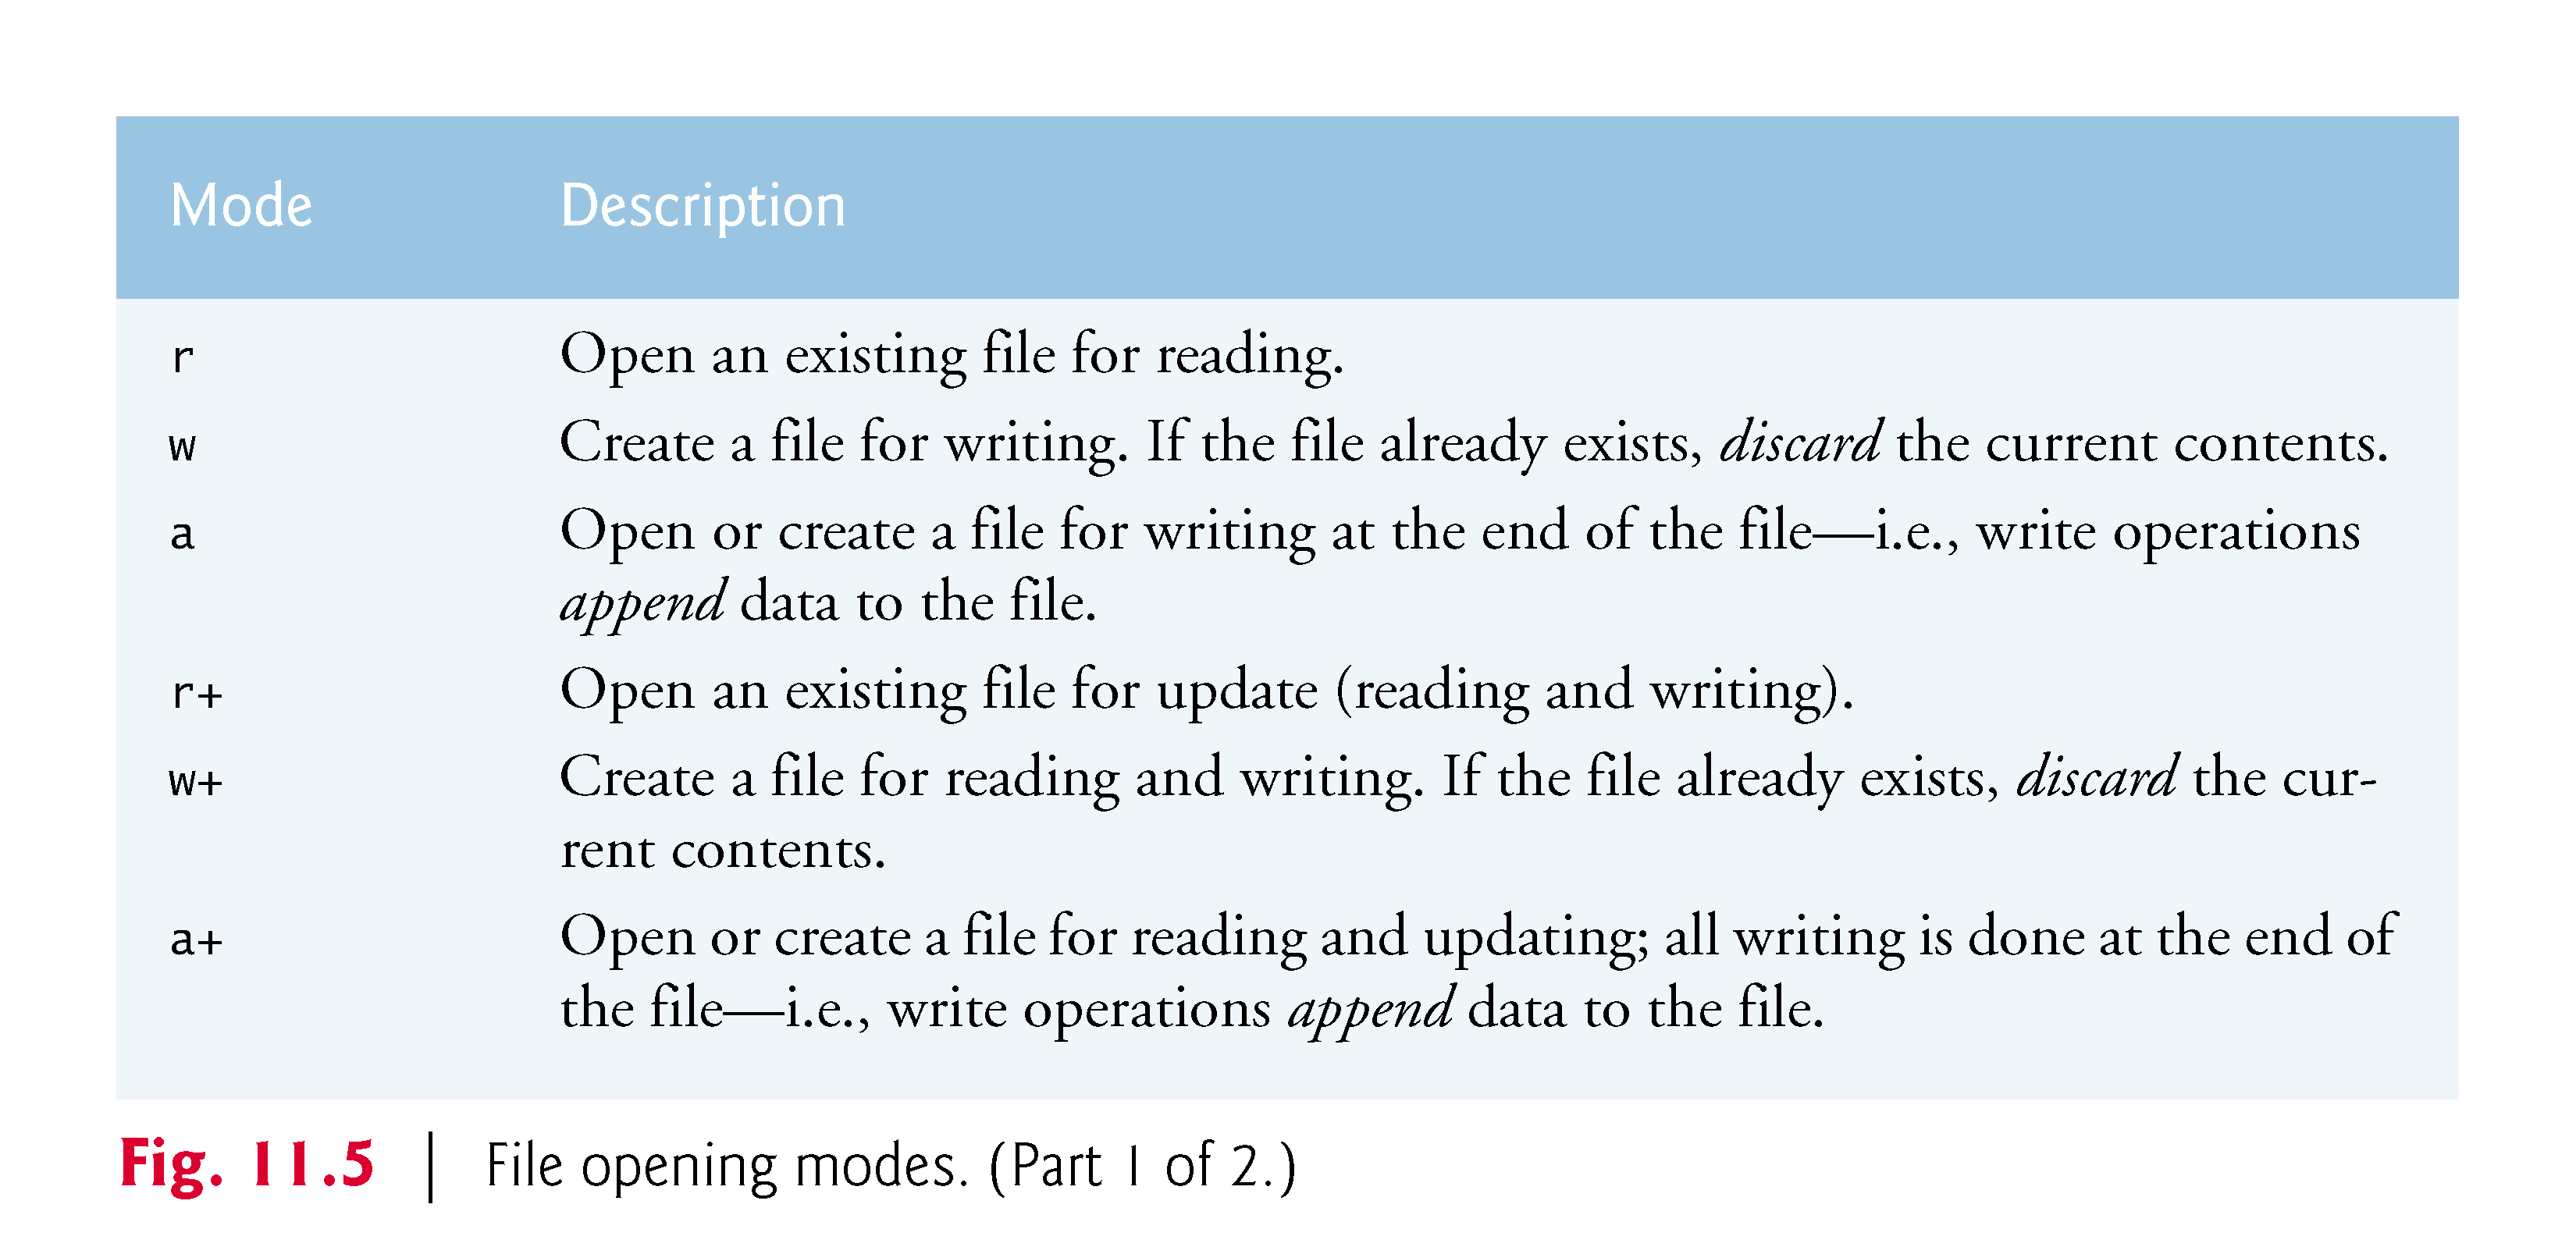
\includegraphics[scale=0.12]{modes.png}
\end{frame}

\begin{frame}[fragile=singleslide]{\texttt{fclose()}}
Just as a dynamically allocated pointer needs to be freed when it is no longer needed, a file stream must be closed when you're finished with it. 
\begin{lstlisting}[style=C]
int fclose(FILE *stream)
\end{lstlisting}
\begin{itemize}
\item This one's pretty straightforward.  Takes the file stream as an argument.
\item Returns 0 on success, EOF on failure.  
\end{itemize}
\end{frame}

\begin{frame}[fragile=singleslide]{\texttt{fscanf()}}
If you want to treat your file like you are reading information from \texttt{stdin}, consider using \texttt{fscanf()} and \texttt{fprintf()}.
\begin{lstlisting}[style=C]
int fscanf(FILE *stream, const char *format, ...)
\end{lstlisting}
\begin{itemize}
\item While the first argument is the file stream we are reading from, the rest of the arguments are used exactly like \texttt{scanf()}.
\item The return value is the number of input items successfully matched and assigned. 
\begin{itemize}
\item i.e., the number of format specifiers in the format string that were successful.  
\end{itemize}
\end{itemize}
\end{frame}

\begin{frame}[fragile=singleslide]{\texttt{fprintf()}}
\begin{lstlisting}[style=C]
int fprintf(FILE *stream, const char *format, ...)
\end{lstlisting}
\begin{itemize}
\item Writes characters into a file in exactly the manner you would expect.
\item First argument is the filestream.
\item Returns the number of characters written if successful, and a negative number upon failure.
\item nuff said.
\end{itemize}
\end{frame}

\begin{frame}[fragile=singleslide]{\texttt{fread()}}
If repeatedly invoking \texttt{fscanf()} isn't your style, perhaps you'd prefer writing chunks of files directly into arrays?
\begin{lstlisting}[style=C]
size_t fread(void *ptr, size_t size, size_t nmemb, FILE *stream)
\end{lstlisting}
\begin{itemize}
\item \texttt{ptr} is a pointer to the memory block you're writing to.  It needs to be at least as big as \texttt{size*nmemb}
\item \texttt{size} is the size in bytes of each element to be read.  
\begin{itemize}
\item So, using \texttt{sizeof()} would be a good idea!
\end{itemize}
\item \texttt{nmemb} is the number of elements to read, each the size of \texttt{size}.
\item \texttt{stream} is, of course, the file stream.
\item \texttt{fread()} returns the total number of elements successfully read.
\end{itemize}
\end{frame}


\begin{frame}[fragile=singleslide]{\texttt{fwrite()}}
And in reverse...
\begin{lstlisting}[style=C]
size_t fwrite(const void *ptr, size_t size, size_t nmemb, FILE *stream)
\end{lstlisting}
\begin{itemize}
\item \texttt{ptr} is a pointer to the array of elements to be written.
\item \texttt{size} is the size, in bytes, of each element of \texttt{ptr}
\item \texttt{nmemb} is the number of elements to be written.
\item \texttt{stream} is, obviously, our old friend the file stream.  
\item \texttt{fwrite()} returns the total number of elements successfully written to the file stream.  
\end{itemize}
\end{frame}


\begin{frame}[fragile=singleslide]{\texttt{feof()}}
So all this reading from files is fine, but how do we know when we're finished? 
\begin{lstlisting}[style=C]
int feof(FILE *stream)
\end{lstlisting}
\begin{itemize}
\item \texttt{feof()} tests to see if the file stream has reached the end of the file.
\item Input is the file stream (naturally)
\item Output is non-zero if the end of the file has been reached, zero otherwise.  
\end{itemize}
\end{frame}

\begin{frame}{An Example!}
\center
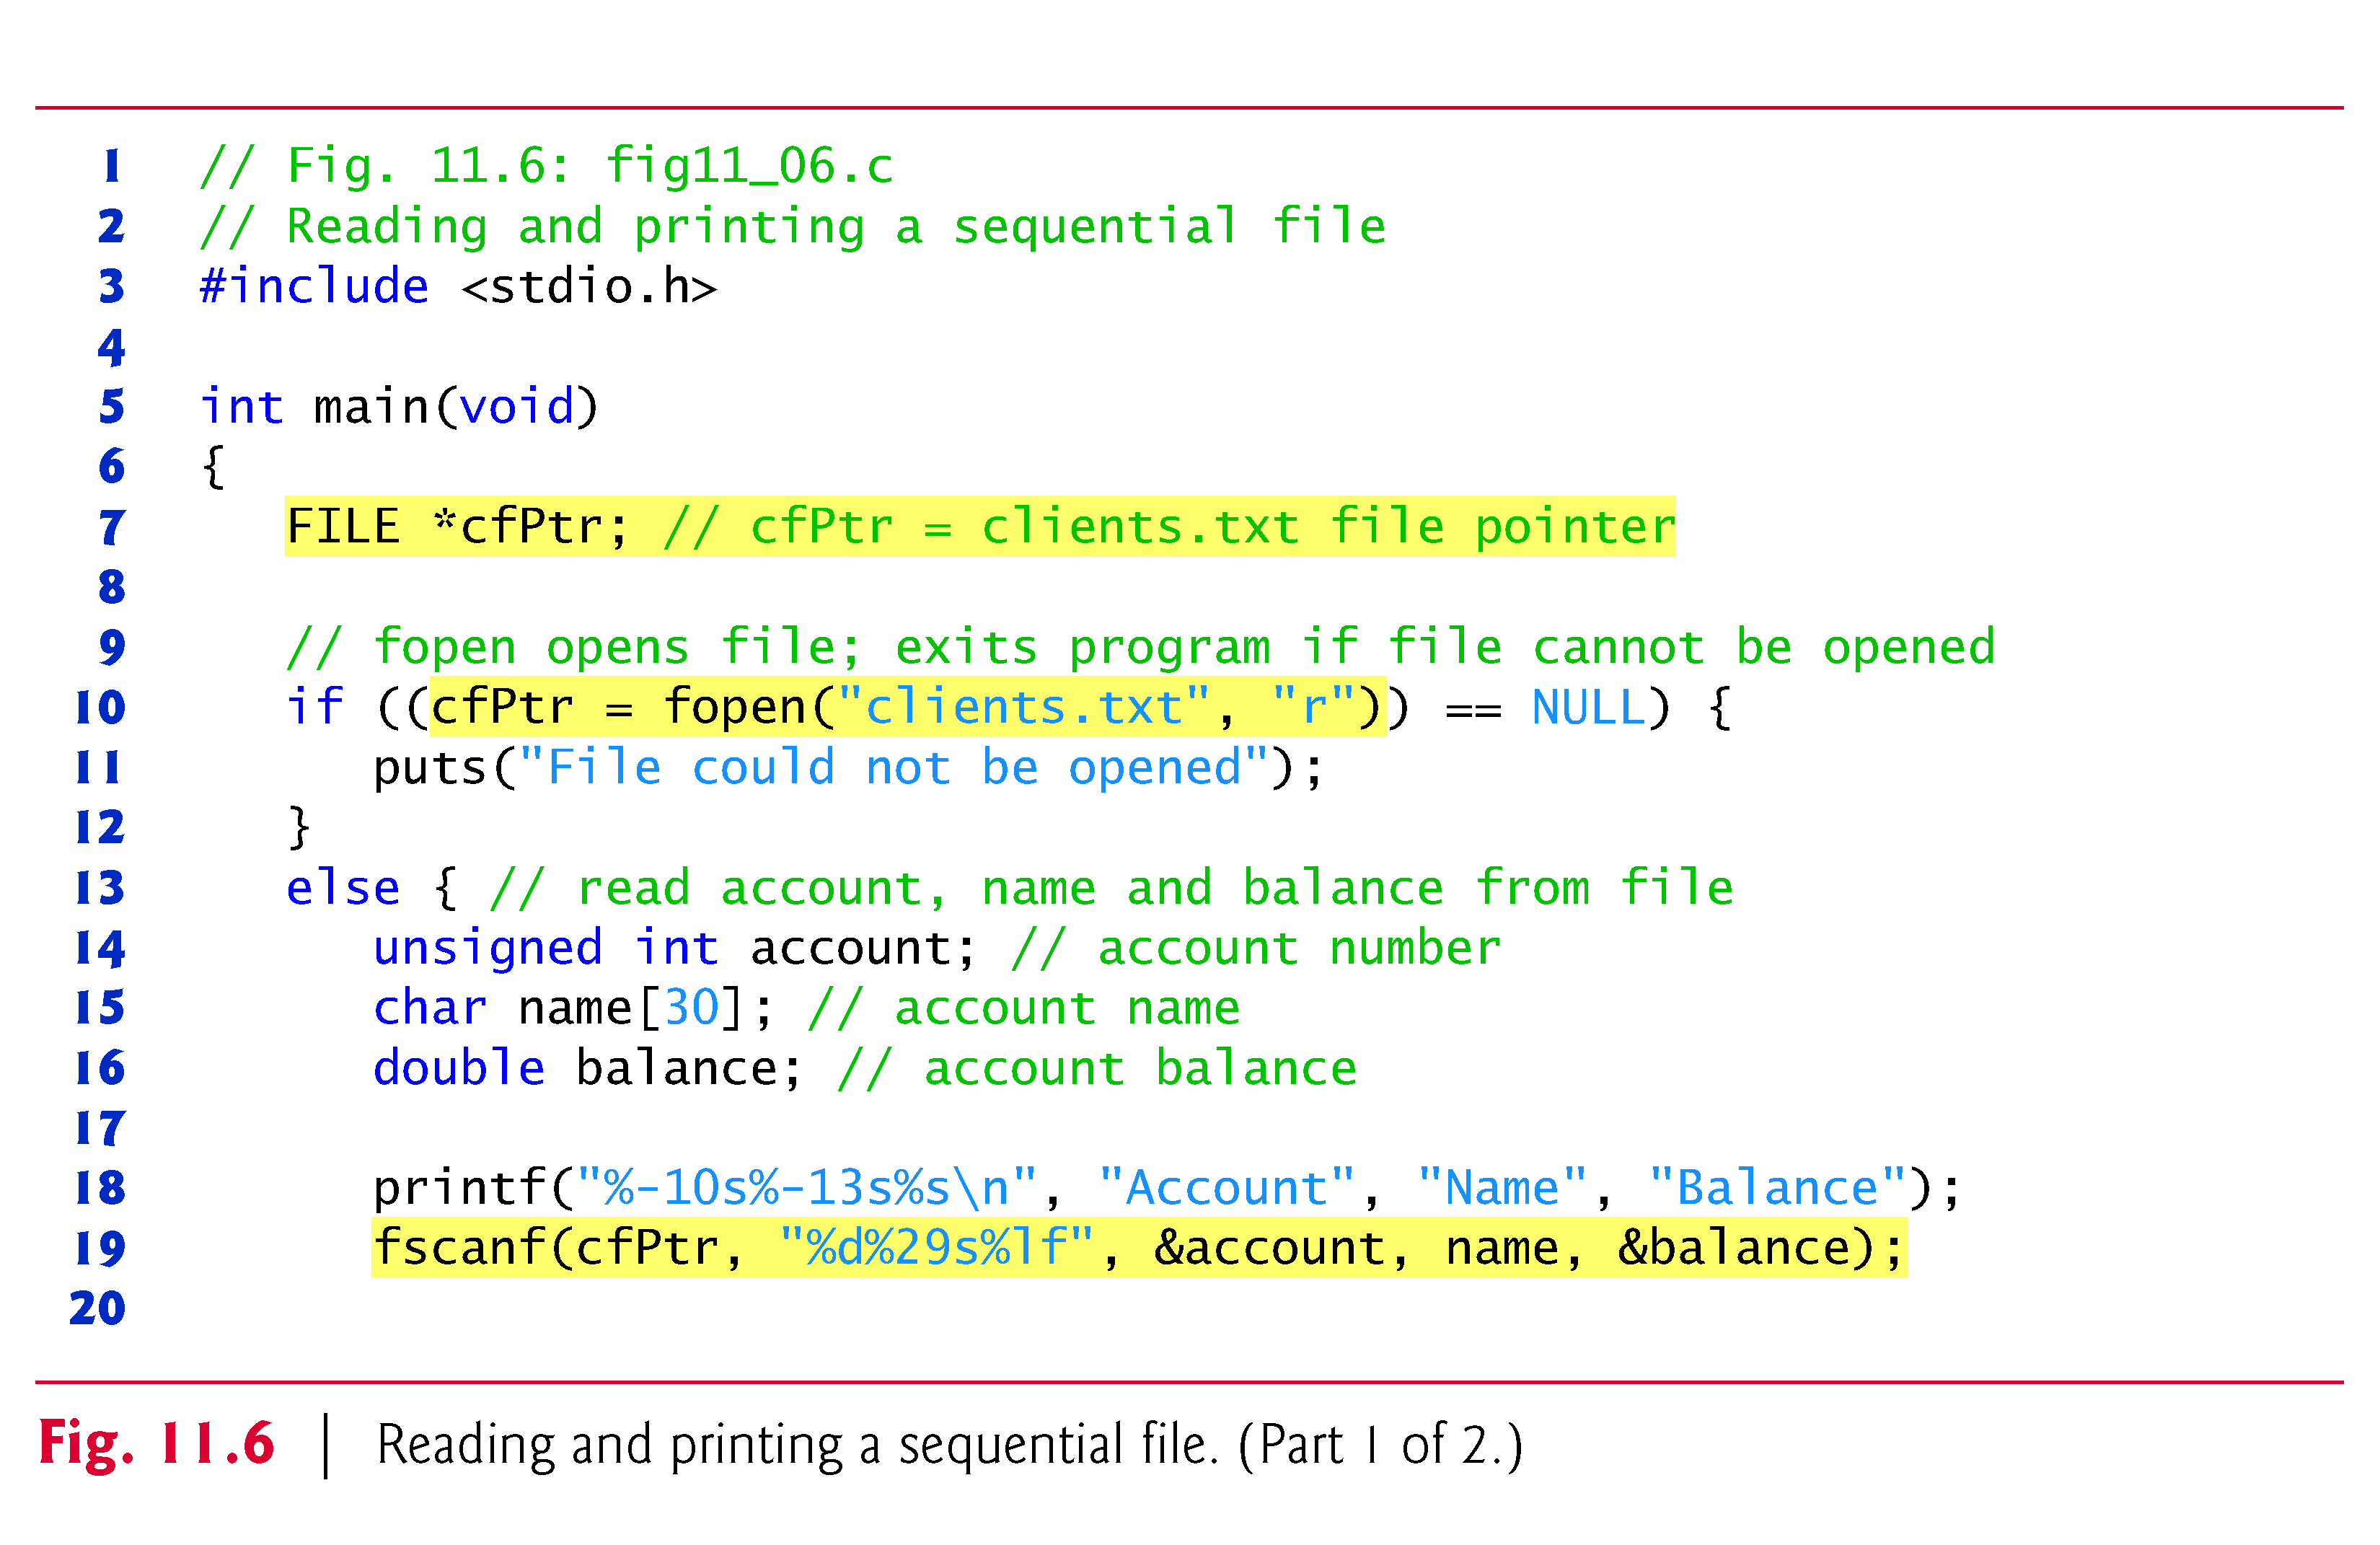
\includegraphics[scale=0.12]{ioex.png}
\end{frame}

\begin{frame}{An Example! (cont.)}
\center
\includegraphics[scale=0.12]{ioex2.png}
\emph{Cue Demo!}
\end{frame}

% \begin{frame}{The Last Slide Comic}
% \center
% 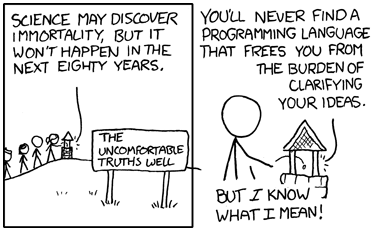
\includegraphics[scale=0.6]{uncomfortable.png}
% \end{frame}

\section[Acknowledge]{Acknowledge}
\begin{frame}{Acknowledge}
\center
\vspace{8em}
The contents of these slides were liberally borrowed (with permission) from slides from the Summer 2021 offering of 1XC3 (by Dr. Nicholas Moore).  
\end{frame}


\end{document}
